\documentclass[fleqn]{scrbook}
\usepackage[latin1]{inputenc}
\usepackage{latexsym}
\usepackage[german]{babel}
%\usepackage{ngerman}
\usepackage[a4paper]{geometry}
\usepackage[sumlimits]{amsmath}
\usepackage{graphicx}
\usepackage{pst-all}
\usepackage{multido}
\usepackage{glossar}
\usepackage{expdlist}
%\usepackage{nomencl}
\pagestyle{headings}
\usepackage{color}
\usepackage{keyval}
\usepackage{listings}
% Gleitobjekte erst nach Definition einf�gen
%\usepackage{flafter}
%\usepackage{charter}
%\geometry{textwidth=17cm, textheight=22cm} 
\parindent0em
\pagenumbering{arabic}

\renewcommand{\glshead}{\chapter*{Glossar}}


\newcommand{\todo}[1]{\hspace{0.5cm}\textbf{\textcolor{red}{TODO}: #1}\hspace{0.5cm}}

\newenvironment{notizen}
{%


\textbf{\textcolor{blue}{Notizen:}}\newline\textbf{\textcolor{blue}{$|^{---}$}}\begin{quote}
}%
{%
  \end{quote}
  \textbf{\textcolor{blue}{$|_{---}$}} \newline
}%

\makeatletter
% args are: width,height,caption,label
\newcommand{\picturehere@caption}{false}
\newcommand{\picturehere@label}{false}
\define@key{picturehere}{caption}[false]{
  \renewcommand{\picturehere@caption}{#1}}
\define@key{picturehere}{label}[false]{
  \renewcommand{\picturehere@label}{#1}}
\newenvironment{picturehere}[4]%
{%
 \setkeys{picturehere}{caption = #3, label = #4}
  \begin{figure*}[h]%
    \begin{center}%
      \begin{minipage}[b]{.3\linewidth}%
        \psset{xunit=1cm,yunit=1cm,runit=1cm}%
        \begin{pspicture}(#1,#2)%
}%
{%
        \end{pspicture}%
      \end{minipage}%
    \end{center}%
    \caption{\picturehere@caption}%
    \label{\picturehere@label}%
  \end{figure*}%
}
\makeatother

%parameters: Bezeichnung, Referenz, ps-Datei
\newcommand{\importgnuplotps}[3]{
  \begin{picturehere}{1}{10}{\mbox{#1}}{#2}
    \includegraphics[bb=530 310 730 600,scale=0.55,angle=-90]{#3}
  \end{picturehere}
}

%parameters: Bezeichnung, Referenz, ps-Datei
\newcommand{\importsmallgnuplotps}[3]{
  \begin{picturehere}{1}{7}{\mbox{#1}}{#2}
    \includegraphics[bb=530 310 730 600,scale=0.4,angle=-90]{#3}
  \end{picturehere}
}

\newcommand{\pubsubrss}{Pub/Sub-RSS }


%%% Local Variables: 
%%% mode: latex
%%% TeX-master: "diplomarbeit"
%%% End: 


\includeonly{einleitung,grundlagen,rss_mittels_verteiltem_pubsub,adaptive_informationsverteilung,experimente,anhang,glossar}

%\title{Adaptive Informationsverbreitung mittels RSS und Publish/Subscribe \\[2cm]\textnormal{Diplomarbeit}}
%\author{Friedemann Zintel}
%\date{\today}

\begin{document}
%\sffamily

%\maketitle

\bibliographystyle{alpha}
%\bibliographystyle{plain}

\frontmatter

\begin{titlepage}
  \begin{center}
    \vspace*{2.5cm}
     \textbf{{\LARGE Diplomarbeit}}\par
    \vspace{1.25cm}
    {\linespread{1.85}\selectfont \textsf{\textbf{{\huge Adaptive Informationsverbreitung mittels RSS und Publish/Subscribe}}}\par}
    \vspace{2.25cm}
    \textnormal{{\Large Friedemann Zintel}}\par
    \vspace{0.75cm}
    {\Large \today}
    \newpage
    \vspace*{6cm}
    {\linespread{1.5}\selectfont \textnormal{{\Large Die selbst�ndige und eigenh�ndige Anfertigung versichere ich an Eides Statt.}}\par}
    \vspace{5cm}
    \textbf{\underline{\hspace{7cm}}}\par
    \textbf{{\Large Berlin, den / Unterschrift}}
  \end{center}
\end{titlepage}

\setcounter{tocdepth}{2}
\setcounter{secnumdepth}{2}
\tableofcontents
\listoffigures
\listoftables

\mainmatter

\chapter{Einleitung}
Der Austausch von Informationen hat seit jeher eine gro�e Bedeutung in menschlichen Gemeinschaften. Das Internet stellt ein Medium dar,
Informationen relativ schnell und leicht zur Verf�gung zu stellen, auszutauschen und zu verbreiten. Zu diesem Zweck sind im Laufe der
Zeit verschiedene Internet-Dienste entwickelt worden. Private Informationen k�nnen als Email (elektronische Post) versendet werden.
Um Informationen einer breiten �ffentlichkeit zug�nglich zu machen, findet die M�glichkeit, diese auf Webseiten zu pr�sentieren, h�ufig Anwendung.
F�r statische Informationen, die keinem stetigen Wechsel unterliegen, ist dies ein geeignetes Verfahren.
Da im Internet pr�sentierte Informationen in zunehmendem Ma�e einen stark dynamischen Charakter aufweisen (z. B. Nachrichten-Schlagzeilen, B�rsennachrichten), 
sind Konzepte entwickelt worden, Interessenten �ber deren inhaltliche �nderungen zu unterrichten. Ein allgemeines Kommunikationsmodell, welches diesem Zweck gerecht
wird, ist Publish/Subscribe.

\section{Motivation}
Im Kommunikationsmodell von verteiltem Publish/Subscribe (kurz: Pub/Sub bzw. Pub/\-Sub-System) finden sich drei
Parteien: \glqq Publisher\grqq{} stellen Informationen �ffentlich zur Verf�gung; \glqq Subscriber\grqq{} interessieren
sich f�r bestimmte Informationen und k�nnen diese abonnieren (subskribieren);
\glqq Message-Broker\grqq{} (kurz: \glqq Broker\grqq) sorgen f�r die Sammlung und Weiterleitung von Notifikationen (Benachrichtigungen) an die Subscriber.
Aufgrund der indirekten Verbindung zwischen Subscribern und Publishern �ber die Broker brauchen sich Publisher nicht um eine Vielzahl von
Interessenten zu k�mmern.
Zudem l�sst die broker-seitige Ansammlung einer Reihe von Informationen die Definition von Filtern zu, durch die
anbieter�bergreifend Informationen seitens der Subscriber abgefragt werden k�nnen.\\

RSS (Really Simple Syndication) z�hlt zwar zu den Pub/Sub-Systemen jedoch nicht zu den verteilten push-basierten, wie sie oben beschrieben wurden,
denn es folgt dem klassischen Client/Server-Ansatz.
Es handelt sich um zentralisiertes Polling, Message-Broker sind hierbei nicht vorgesehen:
auf einer Webseite wird ein RSS-Feed (aktueller Beitrag) vom RSS-Server als XML-Datei abgelegt.
Ein Feed ist einem Thema (Kanal bzw. Channel) zugeordnet und beinhaltet
verschiedene Eintr�ge (z.B. Nachrichten-Schlagzeilen). Interessenten bzw. Nutzer k�nnen nun diese Feeds
herunter laden. Da nicht vorhersehbar ist, zu welchem Zeitpunkt eine Aktualisierung der Feeds seitens des Servers erfolgen wird,
m�ssen die Nutzer in regelm��igen
Zeitabst�nden beim Server nachfragen, um �ber Neuigkeiten informiert zu sein (Polling). Die Definition von Filtern ist nicht vorgesehen,
d.h. Nutzer erhalten den kompletten Feed und m�ssen
sich notfalls bei vielen verschiedenen Servern subskribieren, um eine gro�e Auswahl an Informationen zu einem bestimmten Thema zu erhalten.
RSS-Feeds sind �ber die Channel zwar themenbasiert organisiert (vgl. \cite{LiuVenSirer:2005:MeasureRSSPubSub}), jedoch wird die inhaltlich thematische
Zuordnung auf Server-Seite vorgenommen. Eine thematische Filterung 
aus Nutzersicht auf h�herer Ebene kann lediglich lokal auf Nutzerseite erfolgen.\\
Das st�ndige Abfragen des Servers durch m�glicherweise hunderttausende von Abonnenten f�hrt zu einer
starken server-seitigen Last (vgl. \cite{SandlerEtAl:2005:FeedTree},
\cite{Hicks:2004:RSSBandwith}).
M�chte ein Nutzer eine mit dem Publisher m�glichst synchronisierte Aktualisierung der Feeds erreichen, so muss er die Polling-Rate
hoch setzen. Dies bedeutet wiederum eine h�here Server-Belastung. Um eine hohe Belastung durch hohe Polling-Raten zu unterbinden, haben Server die
M�glichkeit, einen Nutzer (abgrenzbar durch seine IP-Adresse), dessen Polling-Rate zu hoch ist, vor�bergehend zu blocken.
Dadurch ist der Grad der Aktualit�t der RSS-Feeds begrenzt.
Beispiele f�r die (RSS-basierten) Datenmengen, die pro Tag von einzelnen Servern �bermittelt werden m�ssen, finden sich
in \cite{SandlerEtAl:2005:FeedTree}.

\section{Ziele der Arbeit}
Um eine Lastverteilung, besonders auch (und damit) eine potentiell gr��ere Aktualit�t der Informationen und eine h�here Flexibilit�t in Bezug
auf die Auswahl der Informationen seitens der Nutzer zu erreichen, bietet es
sich an, ein push-basiertes Publish/Subscribe-System einzusetzen. RSS-Server k�nnten als Publisher fungieren und neue Feeds eigenm�chtig an ihre lokalen Broker
�bermitteln, welche die Feeds ihrerseits an Nutzer (Subscriber) weiterleiten. Dies w�rde jedoch bedeuten,
dass sowohl auf Nutzer- als auch auf RSS-Server-Seite die schon bestehenden Anwendungen durch neue ersetzt werden m�ssten oder entsprechende Software
installiert werden m�sste.
Solch ein Ansatz w�rde sicherlich auf
Akzeptanzschwierigkeiten sto�en. Au�erdem w�rde der Aktualit�tsgrad hier wie auch bei dem Ansatz unten mit nur einem Poller von dem Overlay-Netz abh�ngen
und k�nnte ung�nstig ausfallen! Um dies zu verhindern, bietet sich folgendes Konzept an: Die Rolle der RSS-Server bleibt bestehen und �ndert sich nicht.
Nutzer entsprechen sowohl den Publishern als auch den Subscribern.
In der Rolle des Publishers erfragt ein Nutzer den aktuellen Feed beim
RSS-Server und speist ihn in das Netz ein bzw. �bermittelt ihn an seinen lokalen Broker.
Dieser sorgt daf�r, dass der Feed an alle Broker weitergeleitet wird, zu denen Subscriber verbunden sind, die sich f�r diesen interessieren.
In der Rolle eines Subscribers erh�lt ein Nutzer einen Feed von
einem Broker. F�r einen Nutzer gibt es also zwei M�glichkeiten einen Feed zu erhalten: direkt vom RSS-Server oder �ber das Netzwerk.
Um eine Server-Entlastung zu erreichen, w�rde es ausreichen, nur
einen Publisher zu definieren, welcher die Feeds in das System einspeist. Alle �brigen Nutzer/Subscriber w�rden
den Feed �ber das Netzwerk erhalten,
wodurch weniger Anfragen beim RSS-Server auftreten w�rden. Doch
dieses Konzept ginge auf Kosten der Aktualit�t der Feeds, da es m�glicherweise sehr lange dauert, bis ein Feed einen Subscriber erreicht (abh�ngig von der
Struktur des Overlay-Netzes).
Es sollte also verschiedene Publisher geben, welche Feeds in das Netzwerk einspeisen und die geeignet im Overlay-Netzwerk positioniert sind.
Die Publisher m�ssen sich untereinander koordinieren, welche von
ihnen den n�chsten Feed herunter laden. Sind es zu viele Publisher, so f�hrt das wiederum zu einer Mehrbelastung des Servers. Es gilt also, ein Optimum
zwischen Aktualit�tsgrad und Server-Belastung zu finden.\\
Ziel dieser Arbeit ist es, ein hohes Update-Intervall ohne Blockierung zu erreichen, indem sich die Publisher beim Polling abwechseln.
Dies kann den Grad an Aktualit�t der Feeds erh�hen.\\

Die Ausarbeitung eines solchen Systems soll folgende Weiterentwicklung erm�glichen: RSS-Feeds k�nnen mit Hilfe von Filtern, welche durch Subscriber
definiert werden,
schon auf der Broker-Ebene gefiltert werden (Filter werden von Brokern an
Nachbarbroker weitergeleitet). Die Filterung kann anbieter�bergreifend wirken, da sich Feeds von unterschiedlichen
RSS-Servern an einem Broker sammeln. Um eine genaue Analyse der Feeds bez�glich der angegebenen Filter zu erm�glichen, wird die inhaltsbasierte Filterung
(content-based filtering, \cite{Muehl:2001:GenericConstraints}) favorisiert. Hierf�r ist es notwendig, nicht nur die Feeds selbst, sondern
auch die durch sie referenzierten Daten herunterzuladen, um sie in den Filtervorgang mit einzubeziehen.
Die Filterung der Feeds auf Broker-Ebene erm�glicht den Subscribern eine
inhaltsorientierte Sichtweise auf Subskriptionen im Gegensatz zur bisherigen anbieterorientierten Sichtweise.\\

Um diese Arbeit in angemessenem Rahmen zu halten, werden wir auf die Umsetzung von Filtertechniken nicht weiter eingehen, schaffen jedoch eine Basis f�r
weitere Entwicklungen in dieser Richtung. Als Ausgangspunkt f�r Erweiterungen verwenden wir die
Filtertechnik des \glqq floodings\grqq{} (siehe \cite{MuFiBu:2002:FilterSimilarities}).\\

Vorteile des genannten Ansatzes gegen�ber anderen Ans�tzen (wie z.B. FeedTree, siehe \cite{SandlerEtAl:2005:FeedTree}) sind:
\begin{itemize}
  \item Die L�sung kann sich problemlos in ein bestehendes RSS-System integrieren, d.h. es ist keine neue Anbieter-Software
        f�r RSS-Server n�tig.
  \item Bei geschickter Umsetzung kann auch die Client-Software weiter verwendet werden (z.B. Abfangen der Anfragen durch einen Proxy).
  \item Eine komplette Neukonstruktion eines Pub/Sub-Systems ist nicht notwendig, auf schon bestehende Systeme kann zur�ckgegriffen und aufgebaut werden
        (z.B. RE\-BE\-CA \cite{MuFiBu:2001:ArchFrameECommApp}).
\end{itemize}

Im Verlauf der Arbeit soll eine angemessene L�sung f�r die oben beschriebene Zielsetzung gefunden werden. Des Weiteren soll eine Simulationsumgebung implementiert
werden, um die entwickelten Algorithmen umzusetzen, zu evaluieren und zu demonstrieren.

\section{wissenschaftlicher Beitrag}
Im Lauf der Arbeit entwickeln wir zwei voneinander relativ unabh�ngige Verfahren:
\begin{itemize}
\item ein Abstimmungsverfahren f�r Klienten bez�glich des n�chsten Zugriffs auf einen Server, welches gegen�ber hohen Nachrichtenlaufzeiten und Knotenausf�llen
  tolerant ist, ohne zu einem stark erh�hten Netzwerkverkehr durch zus�tzliche Abstimmungsnachrichten zu f�hren
\item ein Verfahren zur Adaption von Polling-Raten verschiedener Klienten an den Leistungsgrad eines Servers, das ohne Kenntnis der �brigen Klienten und der
  Gesamtstruktur und -gr��e des Netzwerks auskommt
\end{itemize}
Diese Verfahren wurden zwar in Hinsicht auf RSS entwickelt, sie lassen sich aber auch auf andere �hnlich gestaltete bzw. ereignisbasierte Systeme �bertragen.
Zudem lassen sich die Algorithmen durch geringf�gige Modifikationen auch an
paketorientierte �bertragungstechniken (z. B. UDP) anpassen, obwohl wir diese Verfahren f�r eine datenstrombasierte �bertragungsmethode (TCP) entworfen haben.

\section{Aufbau der Arbeit}
In Kapitel \ref{Abschnitt:Grundlagen} geben wir zun�chst einen �berblick �ber ausgew�hlte Grundbegriffe und Verfahren, soweit sie f�r diese Arbeit von Bedeutung
sind. Im weiteren Verlauf der Arbeit werden wir Begriffe aus diesem Kapitel referenzieren.\\

Kapitel \ref{Abschnitt:RSS_mittels_verteiltem_pubsub} befasst sich mit RSS und der designbezogenen Problematik im Kontext einer gro�en Nutzergemeinde. Wir werden
die schon angesprochenen Ziele unserer Arbeit genauer formulieren und problematische Aspekte bei ihrer Umsetzung beleuchten. Zuletzt geben wir einen kurzen
�berblick �ber Arbeiten, die sich auf vergleichbare oder andere Weise diesem Thema zugewandt haben.\\

In Kapitel \ref{adapt_informationsverteilung} werden wir ein auf unsere Zielsetzung abgestimmtes L�sungskonzept entwickeln. Die Entwicklung erfolgt dabei
schrittweise, und wir werden sie durch die Analyse der gegebenen Begleitumst�nde motivieren.\\

Kapitel \ref{c:implementierung} besch�ftigt sich mit der Implementierung der entwickelten Simulationsumgebung. Wir stellen die wichtigsten Klassen vor, geben einen
�berblick �ber die wichtigsten Methoden und ihr Wechselspiel und erl�utern die Parametrisierung der Software.\\


In Kapitel \ref{c:experimente} stellen wir Experimente vor, mit deren Hilfe wir die entwickelten Algorithmen getestet und evaluiert haben. Die Ergebnisse werden
durch geeignete Graphiken und Diagramme erl�utert.\\

Kapitel \ref{Abschnitt:Zusammenfassung} fasst sowohl die geleistete Arbeit als auch die Ergebnisse zusammen und f�hrt eine abschlie�ende Bewertung durch.
Dar�ber hinaus werden wir einen Ausblick auf m�gliche Erweiterungen zu den entwickelten Verfahren geben.


%%% Local Variables: 
%%% mode: latex
%%% TeX-master: "diplomarbeit"
%%% End: 

\chapter{Grundlagen}
In diesem Kapitel werden wir die f�r das Verst�ndnis des weiteren Textes notwendig erscheinenden technischen Grundlagen erl�utern.
\chapter{Publish/Subscribe}
%\section{Andere Arbeiten}
\section{Peer-To-Peer-Systeme}
\section{Timer}
\label{css:timer}
Ein wichtiger Bestandteil der im weiteren Verlauf der Arbeit vorgestellten Verfahren sind Timer. Daher stellen wir
zun�chst dar, was unter dem Begriff \glqq Timer\grqq{} zu verstehen ist und welche Problematiken sich im Umgang mit Timern ergeben.\\

Bei der Kommunikation zwischen Computern werden Informationen im allgemeinen in einzelne Datenpakete eingeteilt und zwischen
den beteiligten Computern ausgetauscht. Ein Timer ist ein Mechanismus, um in Computer-Kommunikationsnetzen Fehler erkennen zu k�nnen \cite{18216},
welche bei der Kommunikation zwischen Computern auftreten. Diese Fehler k�nnen im einzelnen Verluste von Datenpaketen, das Zusammenbrechen
von Kommunikationskan�len oder indirekt eine Verst�mmelung der �betragenen Informationen bezeichnen. Dabei arbeitet ein Timer wie eine Alarm-Uhr:
nach einer vordefinierten Zeit l�uft der Timer ab. In der Annahme, dass ein bestimmtes Ereignis innerhalb dieser
vordefinierten Zeit zu geschehen hat (im Regelfall eine Antwort des Kommunikationspartners), deutet ein abgelaufener Timer auf
einen aufgetretenen Fehler hin. Hierbei ergeben sich erste Probleme: ist die Zeitspanne bis zum Ablauf eines Timers zu lang,
so wird ein eventuell aufgetretener Fehler zu sp�t erkannt. Ist die Zeitspanne dagegen zu kurz, so kann dies einen falschen Alarm zur Folge haben.
Um ein optimales Leistungsverhalten zu erzielen, wird ein Gleichgewicht zwischen diesen gegens�tzlichen Zielen angestrebt.\\

Verschiedene Timer werden bei Kommunikationsprotokollen (Bsp. TCP, siehe Abschnitt \ref{staukontrolle_tcp}) verwendet, um verschiedenartige
Formen der Kommunikationsst�rung zu erkennen. So sorgt ein \glqq retransmission-timer\grqq{} f�r das wiederholte Aussenden von eventuell verloren gegangenen
Datenpaketen. Dagegen gibt ein \glqq death-timer\grqq{} Auskunft �ber den Zusammenbruch einer Datenverbindung \cite{18216}. Die Zeitspannen
(\glqq Timeout-Intervalle\grqq{}) werden dabei je nach Timer unterschiedlich gesetzt. Um ein Gleichgewicht zwischen der Reduzierung falscher Alarme
und der rechtzeitigen Erkennung aufgetretener St�rungen zu erreichen, werden die Timeout-Intervalle meistens dynamisch und situationsabh�ngig
bestimmt. Folgende Situationen k�nnen nach Zhang \cite{18216} beispielsweise f�r das Ablaufen von retransmission-timern urs�chlich sein:
\begin{enumerate}
\item Ein Datenpaket hat den den Sender noch nicht verlassen (aufgrund eines beispielsweise blockierten Netzwerks), befindet sich aber bereits
  in einer tieferen Anwendungsschicht.
\item Das Timeout-Intervall ist k�rzer als die Zeit bis zu einer positiven Antwort vom Empf�nger.
\item Ein Datenpaket hat den Empf�nger erreicht, die Best�tigungsnachricht ging jedoch verloren.
\item \label{En:Congestion} Ein Datenpaket wurde an einem Vermittlungsknoten (Gateway) aufgrund von Datenstau verworfen.
\item \label{En:Channelerror}Ein Datenpaket wurde augrund eines Fehlers im �bertragungskanal verworfen.
\item Das Netzwerk wurde partitioniert oder der Empf�nger-Knoten ist ausgefallen.
\end{enumerate}

Nur bei Punkt \ref{En:Channelerror} ist ein unmittelbares und wiederholtes Aussenden notwendig. Punkt \ref{En:Congestion} erfordert zwar
auch ein wiederholtes Aussenden eines Datenpakets, das Setzen des retransmission-timers muss aber mit Bedacht geschehen,
um den urs�chlichen Datenstau nicht noch zu vergr��ern. Zhang beschreibt in \cite{18216} die Problematik bei dynamischer Bestimmung der
Timeout-Intervalle. Techniken zur dynamischen Bestimmung von Timeout-Intervallen werden wir in Abschnitt \ref{staukontrolle_tcp} vorstellen.


 
%%% Local Variables: 
%%% mode: latex
%%% TeX-master: "diplomarbeit"
%%% End: 

\section{Staukontrolle bei TCP}
\label{staukontrolle_tcp}
Seitdem Computer-Netzwerke explosionsartig an Gr��e und Komplexit�t zugenommen haben, hat sich ein Problem verst�rkt bemerkbar gemacht: Datenstau.
Van Jacobson et. al. \cite{jacobson88congestion} schildern die Beobachtung, dass Mitte der 1980er Jahre Internet-Gateways 10\% der
ankommenden Pakete aufgrund von Puffer�berl�ufen verwarfen. Laut seiner Aussage lag dabei das Problem nicht in den Protokollspezifikationen selbst, sondern
haupts�chlich in deren Implementierungen. TCP ist ein verbindungsorientiertes �ber\-tra\-gungs\-pro\-to\-koll, mit dessen Hilfe der Gro�teil
des Netzwerkverkehrs vonstatten geht. Im Laufe der Zeit wurden in TCP Mechanismen eingebaut und verbessert, um Datenstau festzustellen und soweit wie m�glich
zu vermeiden. TCP kontrolliert die Daten�bertragung zwischen Sender und
Empf�nger der Endknoten. Dabei wird gew�hrleistet, dass jedes der einzelnen Datenpakete (die einen Datenstrom formen) den Empf�nger erreicht
und dass die Ordnung der Pakete
innerhalb des Datenstroms bestehen bleibt. Bei Datenstau handelt es sich um Verlust von Datenpaketen. Falls es zu Datenstau kommt, so tritt dieser immer an
Verbindungsknoten (einschlie�lich des Empfangsknotens) auf und kann durch verschiedene Ursachen auf dem Weg zwischen Sender und Empf�nger hervorgerufen werden:
\begin{description}
  \item [Bandbreiten:]
    Unterschiedliche Bandbreiten auf dem Weg zwischen Sender und Empf�nger beeinflussen die �bertragungsgeschwindigkeit einer Verbindung
    nachteilig in der
    Form, dass die ``langsamste'' Leitung (also die mit der geringsten Bandbreite) die
    Gesamt-�bertragungsgeschwindigkeit vorgibt. Trifft eine schnelle Leitung auf eine langsame Leitung, so k�nnen die an der langsamen Leitung ankommenden
    Pakete nicht schnell genug weitergeleitet werden. An diesem Knoten kommt es zum Puffer�berlauf, Datenpakete gehen verloren.
  \item [Anzahl der Verbindungen:]
    An einem Knotenpunkt k�nnen mehrere Verbindungen zusammen kommen, die den Gesamt-Datenfluss an diesem Punkt erh�hen. Auch hier kann es zum Puffer�berlauf
    kommen, so dass Datenpakete verloren gehen.
\end{description}
Damit jedes ausgesandte Paket den Empf�nger erreicht, werden in TCP Best�tigungs-Nachrichten (Acknowledgements, im Folgenden kurz $acks$ genannt) versandt.
Erh�lt der Sender f�r ein gesendetes TCP-Datenpaket kein $ack$, so wird er das Datenpaket erneut senden. Ein wichtiger Bestandteil eines Datenpaketes ist
die Sequenznummer \cite{RFC2581}. Anhand der Sequenznummer kann ein $ack$ eindeutig einem versendeten Datenpaket zugeordnet werden. Innerhalb des $acks$ vermerkt
der Empf�nger ebenfalls, welches Datenpaket er als n�chstes erwartet \cite{RFC793}.
Um eine Staukontrolle zu erreichen wurden einige Algorithmen in TCP integriert (siehe \cite{jacobson88congestion}, wir halten uns dabei an die englischen
Bezeichnungen):
\begin{itemize}
  \item slow-start
  \item roundtrip-time variance estimation
  \item exponential retransmit timer backoff
  \item more aggressive receiver ack policy
  \item dynamic window sizing on congestion
  \item Karn's clamped retransmit backoff
  \item fast retransmit
\end{itemize}

Dabei soll erreicht werden, dass die maximal m�gliche Bandbreite (begrenzt durch die minimale Bandbreite (``bottleneck'') auf dem Verbindungsweg, s. o.) voll
ausgenutzt wird, ohne
dass Pakete verloren gehen; es darf also kein Paket in das Netzwerk eingespeist werden, bevor ein altes Paket entfernt wurde (die Verbindung befindet sich dann im
``Equilibrium'', der Paketfluss ist ``conservative'' \cite{jacobson88congestion}). Im Folgenden wollen wir die wichtigsten der oben genannten Algorithmen
vorstellen. Eine genaue Herleitung und Analyse der Algorithmen geht jedoch �ber den Rahmen dieser Arbeit hinaus.
Wir verweisen auf die entsprechenden Quellen in den Literaturangaben.

\paragraph{more aggressive receiver ack policy:}
\footnote{Hier ist in \cite{jacobson88congestion} nicht eindeutig feststellbar,  worauf sich van Jacobson genau bezieht, da er diese Bezeichnung im weiteren Text
nicht mehr verwendet. Es erschien sinnvoll, die folgende im o. g. Text zu findende Erkl�rung diesem Thema zuzuordnen.}TCP
ist ``self-clocking'': da $acks$ erst nach Erhalt der entsprechenden Datenpakete versendet werden k�nnen, bestimmt die Rate der ankommenden $acks$ die
Rate, mit der weitere Datenpakete ausgesendet werden sollen. Die Senderate passt sich somit automatisch der Bandbreite an.

\paragraph{slow-start:}
Durch das ``self-clocking'' tritt nur beim Start des Datentransfers ein Problem auf, da
hier zun�chst eine feste Rate gew�hlt werden muss. Diese wird zu Beginn relativ niedrig gew�hlt, bzw. ein Staufenster ``congestion window'' ($cngw$) 
bestimmt die Anzahl der Pakete pro Sendevorgang. Bei Start des Transfers oder nach Paketverlust wird die Gr��e des Staufenster auf 1 gesetzt.
F�r jedes $ack$ wird das Staufenster um den Betrag 1 erh�ht. Begrenzt wird dessen Gr��e durch das ``advertised receiver window'',
welches vom Empf�nger festgelegt wird und angibt, wieviele Bytes maximal als n�chstes �bersendet werden sollen. Die Zunahme der Gr��e $w$ des
Staufensters geschieht in der Zeit
$rtt\cdot log_2w$, wobei $rtt$ die ``roundtrip-time'' des letzten versendeten Datenpaketes ist (Zeit zwischen Versenden eines Datenpaketes und Erhalt des
entsprechenden $acks$). Siehe dazu \cite{jacobson88congestion,RFC2581}. 

\paragraph{roundtrip-time variance estimation:}
\label{cssp:tcp_rtt}
$Acks$ k�nnen die Geschwindigkeit des Datenflusses steuern, doch was geschieht, wenn $acks$ aufgrund verloren gegangener Pakete ausbleiben? M�ssen sich
beispielsweise bei voll ausgenutzter Bandbreite pl�tzlich zwei Datenstr�me dieselbe Leitung teilen, kommt es bei gleichbleibender Datentransferrate mit Sicherheit zu
Paketverlusten und somit zu
ausbleibenden $acks$. Der Sender muss einen Timer unterhalten, bei dessen Ablauf das zuletzt gesendete Datenpaket erneut versendet wird (im Folgenden als
``Wiederholung'' bezeichnet). Paketverlust kann auch
durch Besch�digung der Daten w�hrend der �bermittlung auftreten. Nach van Jacobson \cite{jacobson88congestion} liegt die Wahrscheinlichkeit daf�r aber weit
unter 1\%. Daher lassen Timeouts bei gut eingestellten Timern mit sicherer Gewissheit auf Paketverluste schlie�en \footnote{Zur Problematik
bei Timern siehe \ref{css:timer}}. Diese Timeouts werden pro Verbindung dynamisch berechnet; im Folgenden bezeichnet $rto$ das ``retransmission timeout''-Intervall,
also die Zeitdifferenz bis zum n�chsten Aussenden eines Datenpaketes. Entsprechend der TCP-Spezifikation
berechnet sich dieser Wert wie folgt \cite{18216}:
\begin{equation}
  rto=min\{UBound, max\{LBound, \beta \cdot srtt\}\}
\end{equation}
$\beta$ ist dabei ein empirisch ermittelter Varianz-Faktor, $UBound$ und $LBound$ sind untere und
obere Schranke f�r den $rto$, $srtt$ ist die ``smoothed roundtrip time'' und
wird wie folgt ermittelt:
\begin{equation}
  srtt= \alpha \cdot  srtt+ (1 - \alpha) \cdot  rtt
\end{equation} 
$\alpha$ ist ein ebenfalls empirisch ermittelter Gl�ttungsfaktor (``smoothing factor''). Empfohlene Werte sind f�r $\alpha:$ $0.8 \sim 0.9$ und f�r $\beta:$
$1.3 \sim 2$ \cite{18216}.\\
Laut van Jacobson \cite{jacobson88congestion} liegt hierin folgende Problematik: $\beta$ kann sich h�chstens an eine bis zu 30\% gesteigerte Last anpassen. Aber die
Varianz des Wertes $rtt$ steigert sich rapide mit ansteigender Last. Bei
Laststeigerung �ber die 30\%-Marke hinaus kommt es zu versp�teten $acks$. Der jeweilige abgelaufene Timer bewirkt eine Wiederholung des entsprechenden
Datenpaketes, was zu unn�tiger Mehrarbeit des Netzwerkes und zu Bandbreitenverschwendung f�hrt. Daher wird $\beta$ ebenfalls dynamisch berechnet.
Eine Berechnungsmethode findet sich in \cite{jacobson88congestion}.

\paragraph{exponential retransmit timer backoff:}
Um den Datenstau durch mehrfach ausgesandte Pakete nicht noch zu vermehren, muss sich der $rto$ stetig vergr��ern.
Van Jacobson \cite{jacobson88congestion} stellt heraus, dass nur exponentielles Wachstum des $rto$ Erfolg verspricht.
Daher wird nach jedem erneuten Aussenden eines nicht best�tigten Datenpaketes der $rto$ verdoppelt.

\paragraph{dynamic window sizing on congestion:}
Ein Vergr��ern des $rto$ verhindert nur einen zus�tzlichen Datenstau durch erneut ausgesandte Datenpakete. Damit auch die im Anschluss daran neu
ausgesandten Pakete nicht wieder zum Anstieg des Datenstaus f�hren, wird ebenfalls die Gr��e der Staufenster $cwnd$ halbiert (exponentielle Abnahme).
Ausbleibende oder verz�gerte $acks$ geben nur Auskunft �ber auftretenden Datenstau. Sie k�nnen nicht anzeigen, ob die volle Bandbreite einer Verbindung auch wirklich
ausgenutzt wird. Daher sollte die Gr��e der Staufenster nach einem bestimmten Schema angehoben werden. Die Anpassung von $cwnd$ geschieht nach folgendem Prinzip:
\begin{itemize}
  \item Nach jedem Timeout wird $cwnd$ halbiert.
  \item Nach jedem $ack$ f�r neue Daten wird $cwnd$ um $1/cwnd$ erh�ht.
  \item Beim Senden wird das Minimum an Daten von $cwnd$ und dem ``receivers advertised window'' gesendet.
\end{itemize}

Dieser Algorithmus tr�gt zur Stauvermeidung (``congestion avoidance'') bei und besteht parallel zum ``slow-start''-Algorithmus. Van Jacobson gibt in
\cite{jacobson88congestion} ein Auswahlkriterium an, nachdem zustandsabh�ngig zwischen beiden Algorithmen ausgew�hlt wird.

\paragraph{Karn's clamped retransmit backoff:}
\label{csp:karns_algorithmus}
Sequenznummern erm�glichen die Zuordnung eines $acks$ zu dem entsprechenden Datenpaket. Kommt es aufgrund von Timeouts zu Wiederholungen
desselben Datenpaketes, so tritt ein Problem auf, welches Karn und Partridge in \cite{Karn1991} als ``retransmission ambiguity'' bezeichnen:
es kann nicht festgestellt werden, auf welche Aussendung desselben Datenpaketes sich das $ack$ bezieht. Damit ist nicht klar, anhand welches Paketes
sich der $rtt$ bestimmen soll, er wird in jedem Falle nicht verl�sslich sein. Verschiedene Protokollimplementationen behandeln dieses Problem
auf unterschiedliche Weise: teils wird die am l�ngsten zur�ckliegende Aussendung als Grundlage zur Berechnung herangezogen, teils die am k�rzesten zur�ckliegende
Aussendung.\\

Wird die am l�ngsten zur�ckliegende Aussendung  gew�hlt, so k�nnen der $rtt$, damit der $srtt$ und letztlich der $rto$ unverh�ltnism��ig in die H�he schie�en.
In vielen F�llen ist die nachteilige Wirkung nicht besonders gro�, da aufgrund des Datenstaus eine Drosselung der Datentransferrate erw�nscht ist.
Kommt es aufgrund anderer Ursachen zu Paketverlusten (z. B. bei verlustreichen Leitungen durch St�rsignale), so tritt das Gegenteil des gew�nschten Verhaltens
ein: der $srtt$ sinkt auf ein sehr niedriges Niveau, obwohl sich in diesem Falle die Datentransferrate erh�hen sollte.\\

Wird die am k�rzesten zur�ckliegende Aussendung herangezogen, so ist die Wahrscheinlichkeit laut Karn sehr gro�, dass die Zeitfolge zwischen dieser Sendung und dem
ankommenden $ack$ sehr kurz ist, obwohl sich das $ack$ auf eine weiter zur�ckliegende Sendung bezieht. Dies f�hrt zu einer drastischen Reduzierung des $srtt$,
was �berfl�ssige Wiederholungen und damit eine zus�tzliche Verschwendung der Bandbreite zur Folge hat \cite{Karn1991,Jain1986}. Andere Implementationen
lassen den $rtt$ bei Wiederholungen au�er acht. Dies geht gut, solange der $rto$ nicht schneller ansteigt, als der Algorithmus sich adaptieren kann. Ist $\beta$
gut gew�hlt, so ist die M�glichkeit daf�r sehr gering. Tritt dieser Fall dennoch ein, so kommt es (wie im letztgenannten Fall) zu �berfl�ssigen Wiederholungen.\\

Um diesem Problem zu begegnen, schl�gt Karn folgenden Algorithmus vor \cite{Karn1991}:\\
Grunds�tzlich wird der $rto$ nach einem Timeout vergr��ert (``back-off'').
Erreicht ein $ack$ den Sender nach einer Wiederholung eines Datenpaketes, so wird keine Neuberechnung des $rtt$ und $srtt$ vorgenommen. Daf�r wird der neu
ermittelte (``backed-off'') $rto$ als Grundlage f�r die n�chste Wiederholung bzw. f�r die Aussendung des n�chsten Datenpaketes herangezogen. Nur wenn ein $ack$
den Sender ohne vorausgehende Wiederholung erreicht, wird der $rto$ mit Hilfe des nun neu berechneten $srtt$ ermittelt.\\
Die Wahl des neuen $rto$ im Falle einer Wiederholung muss laut Karn so erfolgen, dass der $rto$ gr��er ist als die tats�chliche roundtrip-time. Typischerweise
geschieht die Steigerung des $rto$ exponentiell (entsprechend des ``exponential retransmit timer backoff'', s. o.).

\paragraph{fast retransmit:}
Erreichen den Sender vier identische $acks$ in Folge, so wird der Sender das vom Empf�nger erwartete Datenpaket sofort aussenden, ohne auf das
Ablaufen des Retransmission-Timers zu warten. ``Slow-start'' wird so lange ausgesetzt, bis ein anderes, nicht zu den vorherigen identisches $ack$ den Sender
erreicht  (\cite{RFC2581}). Die identischen $acks$ lassen sowohl darauf schlie�en, dass ein Datenpaket verloren gegangen ist, als auch, dass andere Datenpakete den
Empf�nger h�chstwahrscheinlich erreichen, da die identischen $acks$ sonst ausgeblieben w�ren. Die den identischen $acks$ zugrundeliegenden Datenpakete beeinflussen
das Datenaufkommen nicht mehr, da diese schon die Empf�nger-Queue erreicht haben. Daher geht man davon aus, dass das erneute, schnelle Senden des fehlenden
Datenpaketes das Netz nicht wesentlich im Negativen beeinflusst. ``Fast retransmit'' sollte, muss aber nicht, von einer konkreten TCP-Implementation unterst�tzt
werden.\\

Zus�tzliche Erweiterungen zum TCP in Hinsicht auf hohe Performanz finden sich in \cite{jacobson93tcp}.

%%% Local Variables: 
%%% mode: latex
%%% TeX-master: "diplomarbeit"
%%% End: 

\section{Regelkreise}
\label{regelungstechnik}
Auf dem Gebiet der Regelungstechnik besch�ftigt man sich damit, wie eine Gr��e einen bestimmten vorgegebenen Wert erreichen und halten kann. Bei einer Regelung
finden Kontrollmechanismen
Anwendung, um Wertabweichungen festzustellen und auszugleichen.\\

Die Aufgabe einer Regelung besteht darin, bestimmte Gr��en (Temperatur, Spannung, etc.) auf einen
vorgeschriebenen Wert zu bringen und diesen entgegen allen St�reinfl�ssen konstant zu halten (\cite{Bernstein1998}). Bei der Regelung unterscheidet man zwischen
verschiedenen Gr��en, die zusammen einen Regelkreis bilden: 
\begin{description}
  \item [Regelgr��e $x$] oder auch der Istwert: Gr��e, welche konstant gehalten werden soll und zu diesem Zweck erfasst wird
  \item [F�hrungsgr��e $w$] oder auch Sollwert: vorgegebener Wert, auf den die Regelgr��e eingestellt werden soll
  \item [St�rgr��e $z:$] Gr��e, die die Regelgr��e in unerw�nschter Weise beeinflusst
  \item [Regeldifferenz $x_d:$] Differenz zwischen F�hrungs- und Regelgr��e $x_d=w-x$
  \item [Stellgr��e $y:$] Gr��e, durch welche die Regelgr��e in erw�nschter Weise beeinflusst wird
\end{description}

\begin{picturehere}{1}{4}{Regelkreis}{Abb:Regelkreis}
 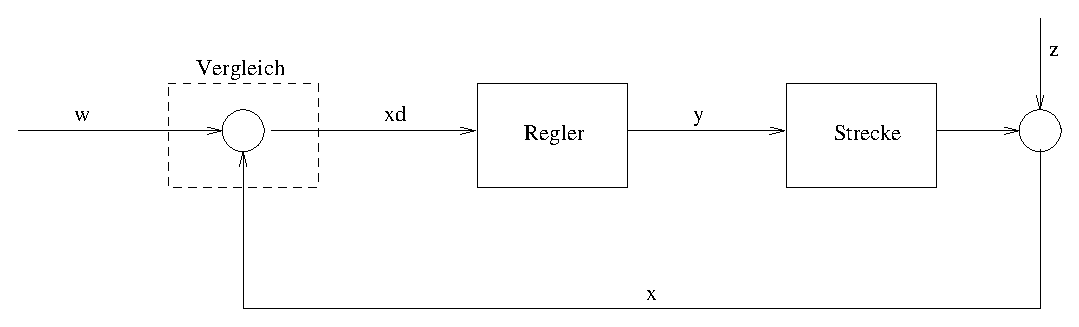
\includegraphics[bb=180 0 682 141,scale=0.75]{Regelkreis}
\end{picturehere}

%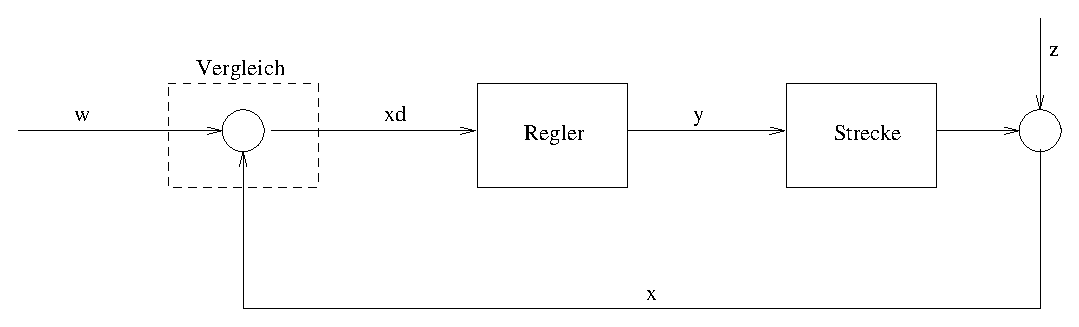
\includegraphics[scale=0.75]{Regelkreis.pstex}

Bild \ref{Abb:Regelkreis} zeigt das vereinfachte Schema eines Regelkreises. Die Regelung basiert auf R�ckkopplung. Bewirkt der Einfluss der St�rgr��e eine
Abweichung der Regelgr��e von der F�hrungsgr��e, so ergibt die Regeldifferenz �ber einen Regler eine Stellgr��e, die entgegengesetzt zur St�rgr��e auf die
Regelgr��e einwirkt. Ziel dabei ist es, die Regeldifferenz auf Null zu bringen.\\
Die Wahl eines geeigneten Reglers h�ngt stark von der Regelstrecke ab. Die Regelstrecke bezeichnet die zu regelnde Anlage oder den zu regelnden Prozess. Wichtig zu
wissen ist, wie die Regelstrecke auf �nderung der Einflussgr��en reagiert. Nach \cite{Bernstein1998} kann man die Regelstrecken grob durch folgende Merkmale 
unterscheiden:
\begin{itemize}
  \item Regelstrecken mit und ohne Ausgleich
  \item Regelstrecken mit und ohne Totzeiten bzw. Zeitgliedern
  \item lineare oder nichtlineare Regelstrecken
\end{itemize}

Bei Regelstrecken mit Ausgleich erreicht die Ausgangs- bzw. Regelgr��e nach einer gewissen Zeit einen stabilen Zustand (Bsp. Raumtemperatur). Existiert kein
stabiler Zustand (Regelstrecke ohne Ausgleich), so �ndert sich bei konstanter Eingangs- bzw. Stellgr��e die Regelgr��e mit
konstanter Geschwindigkeit oder Beschleunigung (Bsp. F�llen eines Wasserbeh�lters). Totzeit bezeichnet eine Zeitverz�gerung, bis sich die �nderung der Stellgr��e
auf die Regelgr��e bemerkbar macht. Bei linearen Regelstrecken folgt die Regelgr��e der Stellgr��e proportional.

Meist liegt eine Kombination dieser Eigenschaften vor. Um die Stellgr��e entsprechend der Regeldifferenz anzupassen, wird ein Regler ben�tigt.

\paragraph{PID-Regler:}
Ein PID-Regler ist ein allgemeiner Reglertyp, der h�ufig f�r Regelungen Verwendung findet. Er ist eine Kombination aus einem P-, einem I- und einem D-Regler.
Ein P-Regler sorgt daf�r, dass (im station�ren Zustand) ein dem Eingangssignal proportionales Ausgangssignal geliefert wird (unter Zuhilfenahme eines
Verst�rkungsfaktors). Ein I-Regler summiert die Regeldifferenz �ber einen gewissen Zeitraum und f�hrt damit eine Integration aus. Je l�nger eine Regeldifferenz
besteht, desto gr��er wird die Stellgr��e. Ein D-Regler reagiert nur auf die �nderungsgeschwindigkeit der Regeldifferenz. Er liefert einen entsprechend starken,
kurzen, positiven Impuls.

Die allgemeine mathematische Gleichung f�r einen PID-Regler lautet wie folgt
(siehe \cite{WBuettner1991}):
\begin{equation}
  u(t)=K_R\left[\quad e(t) \quad + \quad
    \frac{1}{T_I}\int\limits_{0}^{t}e(\tau)d\tau \quad + \quad
    T_D\frac{de(t)}{dt} \quad \right]
\end{equation}

Die einzelnen Gr��en sind:
\begin{description}
  \item [$u(t)$] Stellgr��e
  \item [$e(t)$] Regeldifferenz
  \item [$K_R$] Verst�rkungsfaktor
  \item [$T_I$] Integrationskonstante
  \item [$T_D$] Differentiationskonstante
\end{description}

Es werden nicht f�r alle Regelungen alle Anteile ben�tigt. Durch Weglassen der entsprechenden Anteile erh�lt man die Regler P, PI bzw. PD. Reine P-Regler finden
nur Verwendung bei Regelstrecken linearen Verlaufs. Doch selbst hier zeigt sich, dass bei Regelabweichungen, die durch eine St�rgr��e hervorgerufen werden, die
St�rgr��e lediglich in ihrer Wirksamkeit gemindert werden kann. Eine vollst�ndige Beseitigung tritt nicht ein, da die Regelabweichung selbst notwendig ist, um eine
Verstellung des Stellgliedes vorzunehmen \cite{Bernstein1998}. Mit einem I-Regler kann man die Regelabweichung sehr genau unterbinden, jedoch arbeitet dieser
relativ langsam und neigt zu Schwingungen. Die Vorteile beider Reglertypen vereint der PI-Regler. Reine D-Regler finden in der Praxis keine Verwendung, da sie bei
stabiler Regelgr��e nicht in den Regelvorgang eingreifen k�nnen. Die Kombination mit einem P-Regler (also ein PD-Regler) bewirkt ein schnelleres Anspringen der
Regelung bei pl�tzlicher Regelabweichung im Vergleich zu einem reinen P-Regler.

%%% Local Variables: 
%%% mode: latex
%%% TeX-master: "diplomarbeit"
%%% End: 


%%% Local Variables: 
%%% mode: latex
%%% TeX-master: "diplomarbeit"
%%% End: 

\chapter{RSS mittels verteiltem Publish/Subscribe}
\chapter{RSS}

\section{Das Verteilungsschema bei RSS und seine Problematik}
Ein Problem bei Dienstapplikationen im Internet ist eine starke Serverbelastung zu Sto�zeiten.
Die Masse der Anfragen an einen Server kann dazu f�hren, dass dieser der zeitgerechten Beantwortung nicht mehr nachkommen kann.
Im schlimmsten Fall
k�nnen einige Anfragen gar nicht beantwortet werden, da die Masse der Anfragen die zur Verf�gung gestellte Verarbeitungsapazit�t des Servers
�bersteigt. Ein Server unterh�lt im Regelfall eine Warteschlange (Queue), in der diejenigen Anfragen vorgehalten werden, welche aufgrund
anderer in Abfertigung befindlicher Anfragen momentan nicht bearbeitet werden k�nnen. Wird die Kapazit�tsgrenze dieser Warteschlange erreicht,
k�nnen weitere �bersch�ssige Anfragen nicht bearbeitet werden, sie werden verworfen.\\

Beim bestehenden Konzept zur Verteilung von RSS-Feeds kann es
vorkommen, dass Subscriber, deren Anfragen sich sehr weit hinten in der Warteschlange eines RSS-Servers befinden, erst sehr sp�t bzw. zu sp�t die gew�nschten
Informationen erhalten. Man denke z.B. an aktuelle B�rsennachrichten, welche im Sekundenbereich aktualisiert werden. Hier kann eine Nachricht
schon als veraltet gelten, erreicht sie den Interessenten einige Sekunden zu sp�t. Subscriber, deren Anfragen den RSS-Server bei bereits
ausgesch�pfter Kapazit�t der Warteschlange erreichen, kommen gar nicht an die gew�nschte Information.\\

Ein weiteres Problem im Zusammenhang mir RSS ist der erh�hte Verbrauch von Bandbreiten durch die �bertragung redundanter Daten. Die klientenseitige
Einstellung hoher Polling-Raten kann die wiederholte �bertragung unver�nderter RSS-Feeds provozieren. Diese zus�tzliche Belastung eines Web-Servers kann dazu
f�hren, dass dieser seiner normalen T�tigkeit nicht mehr zufriedenstellend nachkommen kann \cite{Hicks:2004:RSSBandwith}.
Zudem werden RSS-Feeds an jeden Klienten separat �bermittelt. Gleiche Interessen und nahegelegene Positionierung von Klienten im Internet k�nnen nicht ausgenutzt
werden, bzw. es obliegt Subnetzen durch die Einrichtung von Proxies und/oder Caches diese Vorteile auszunutzen. Um einige der oben genannten Probleme einzud�mmen,
wird ab der RSS-Version 0.92 der Parameter \texttt{cloud} unterst�tzt (siehe Abschnitt \ref{ch_rss}). Mit diesem Parameter kann ein Web-Service definiert werden,
bei dem sich Subscriber registrieren k�nnen, um �ber Aktualisierungen eines RSS-Feeds unterrichtet zu werden (dies wird auch als
\glqq lightweight publish/subscribe\grqq{} bezeichnet \cite{RSSSpecWi2004}). Somit kann unn�tiges Pollen eines RSS-Servers
vermieden werden. Doch k�nnen weitere, oben angesprochene Probleme damit nicht vermieden werden, und es ergeben sich zus�tzliche H�rden:
\begin{itemize}
\item Ein Publisher muss einen Web-Service einrichten, welcher Klienten �ber Aktualisierungen benachrichtigt.
\item Der Web-Service muss m�glicherweise eine Vielzahl von Klienten/Subscribern verwalten.
\item Umfangreichere Filterkriterien als nach bestehenden Kan�len auszuw�hlen, sind nicht m�glich.
\item Es wird nur ein unn�tiges Pollen verhindert. Klienten m�ssen nach wie vor den RSS-Server kontaktieren, um RSS-Feeds zu erhalten. Ein Austausch der Feeds
  unter den Klienten und somit eine Lastverteilung der Datenmengen ist damit nicht m�glich.
\end{itemize}

\section{Ziele}
\label{vs_ziele}
Unser prim�res Ziel ist es, ein Verteilungsschema zu konzipieren, bei dem jeder Subscriber die gew�nschten Informationen zeitgerecht erh�lt.
Die Definition von komplexen Filtern, die die Menge der Informationen einschr�nkt bzw. �ber die bestehenden Kan�le hinaus erweitert, soll erm�glicht werden.
Die sekund�ren Ziele ergeben sich im Verlauf der Arbeit.\\

Je fr�her ein Subscriber die neueste Information, die beim RSS-Server vorliegt, erh�lt, desto gr��er ist ihr Aktualit�tsgrad.
F�hren wir uns kurz vor Augen, welche Faktoren den Aktualit�tsgrad beeinflussen k�nnen. Denkbar sind drei Situationen, die den Aktualit�tsgrad
negativ beeinflussen:
\begin{enumerate}
  \item Anfrage des Subscribers an den RSS-Server kommt sp�t \label{enum:anf_zsp}
  \item Antwort des RSS-Servers erreicht den Subscriber sp�t \label{enum:ant_zsp}
  \item Subscriber erh�lt gar keine Antwort vom RSS-Server \label{enum:k_ant}
\end{enumerate}

Zu \ref{enum:anf_zsp}.: da wir es bei dem bestehenden Pull-Ansatz mit aktivem Polling der Subscriber zu tun haben, bewirkt eine h�here
Polling-Rate eine h�here Chance, dass Anfragen den RSS-Server mit geringer Verz�gerung erreichen (bezogen auf neue vorliegende Informationen).
Gegenma�nahme w�re also, die Polling-Rate eines Subscribers zu erh�hen, um die Anzahl der Anfragen, die den RSS-Server pro Zeiteinheit erreichen,
zu erh�hen.\\

Zu \ref{enum:ant_zsp}.: zu sp�t erhaltene Antworten k�nnen (abgesehen von langen �ber"-tra"-gungs"-zeiten) darauf zur�ckzuf�hren sein,
dass der RSS-Server mit der Beantwortung nicht nachkommt, seine Queue also zu voll ist. Abhilfe schafft hier eine Drosselung der Anzahl der
Anfragen an den RSS-Server.\\

Zu \ref{enum:k_ant}.: um trotzdem an die gew�nschten Informationen zu gelangen, muss daf�r gesorgt werden, dass der RSS-Server nicht die einzige
Quelle ist, von der jene Informationen bezogen werden k�nnen.\\

Die Ma�nahmen in den Punkten \ref{enum:anf_zsp}. und \ref{enum:ant_zsp}. widersprechen sich zun�chst. Eine Erh�hung der Anzahl der Anfragen kann also die Erf�llung
von \ref{enum:ant_zsp}. mit sich f�hren.
Zudem kann dies sogar die Erf�llung von \ref{enum:k_ant}. nach sich ziehen: bei einigen RSS-Servern ist vorgesehen, die
Anfragen von Subscribern, welche in zu geringen zeitlichen Abst�nden auf den RSS-Server treffen, zu blocken. Wir suchen also nach einer L�sung,
bei der sich die drei Punkte nicht gegenseitig negativ beeinflussen bzw. sich die Waage halten.

%%% Local Variables: 
%%% mode: latex
%%% TeX-master: "diplomarbeit"
%%% End: 

\section{Verwandte  Arbeiten}
\todo{f�llen}
\subsection{FeedTree}
\todo{f�llen}

\chapter{Adaptive Informationsverteilung}
\section{Das Verteilungsschema bei RSS und seine Problematik}
Ein Problem bei Dienstapplikationen im Internet ist eine starke Serverbelastung zu Sto�zeiten.
Die Masse der Anfragen an einen Server kann dazu f�hren, dass dieser der zeitgerechten Beantwortung nicht mehr nachkommen kann.
Im schlimmsten Fall
k�nnen einige Anfragen gar nicht beantwortet werden, da die Masse der Anfragen die zur Verf�gung gestellte Verarbeitungsapazit�t des Servers
�bersteigt. Ein Server unterh�lt im Regelfall eine Warteschlange (Queue), in der diejenigen Anfragen vorgehalten werden, welche aufgrund
anderer in Abfertigung befindlicher Anfragen momentan nicht bearbeitet werden k�nnen. Wird die Kapazit�tsgrenze dieser Warteschlange erreicht,
k�nnen weitere �bersch�ssige Anfragen nicht bearbeitet werden, sie werden verworfen.\\

Beim bestehenden Konzept zur Verteilung von RSS-Feeds kann es
vorkommen, dass Subscriber, deren Anfragen sich sehr weit hinten in der Warteschlange eines RSS-Servers befinden, erst sehr sp�t bzw. zu sp�t die gew�nschten
Informationen erhalten. Man denke z.B. an aktuelle B�rsennachrichten, welche im Sekundenbereich aktualisiert werden. Hier kann eine Nachricht
schon als veraltet gelten, erreicht sie den Interessenten einige Sekunden zu sp�t. Subscriber, deren Anfragen den RSS-Server bei bereits
ausgesch�pfter Kapazit�t der Warteschlange erreichen, kommen gar nicht an die gew�nschte Information.\\

Ein weiteres Problem im Zusammenhang mir RSS ist der erh�hte Verbrauch von Bandbreiten durch die �bertragung redundanter Daten. Die klientenseitige
Einstellung hoher Polling-Raten kann die wiederholte �bertragung unver�nderter RSS-Feeds provozieren. Diese zus�tzliche Belastung eines Web-Servers kann dazu
f�hren, dass dieser seiner normalen T�tigkeit nicht mehr zufriedenstellend nachkommen kann \cite{Hicks:2004:RSSBandwith}.
Zudem werden RSS-Feeds an jeden Klienten separat �bermittelt. Gleiche Interessen und nahegelegene Positionierung von Klienten im Internet k�nnen nicht ausgenutzt
werden, bzw. es obliegt Subnetzen durch die Einrichtung von Proxies und/oder Caches diese Vorteile auszunutzen. Um einige der oben genannten Probleme einzud�mmen,
wird ab der RSS-Version 0.92 der Parameter \texttt{cloud} unterst�tzt (siehe Abschnitt \ref{ch_rss}). Mit diesem Parameter kann ein Web-Service definiert werden,
bei dem sich Subscriber registrieren k�nnen, um �ber Aktualisierungen eines RSS-Feeds unterrichtet zu werden (dies wird auch als
\glqq lightweight publish/subscribe\grqq{} bezeichnet \cite{RSSSpecWi2004}). Somit kann unn�tiges Pollen eines RSS-Servers
vermieden werden. Doch k�nnen weitere, oben angesprochene Probleme damit nicht vermieden werden, und es ergeben sich zus�tzliche H�rden:
\begin{itemize}
\item Ein Publisher muss einen Web-Service einrichten, welcher Klienten �ber Aktualisierungen benachrichtigt.
\item Der Web-Service muss m�glicherweise eine Vielzahl von Klienten/Subscribern verwalten.
\item Umfangreichere Filterkriterien als nach bestehenden Kan�len auszuw�hlen, sind nicht m�glich.
\item Es wird nur ein unn�tiges Pollen verhindert. Klienten m�ssen nach wie vor den RSS-Server kontaktieren, um RSS-Feeds zu erhalten. Ein Austausch der Feeds
  unter den Klienten und somit eine Lastverteilung der Datenmengen ist damit nicht m�glich.
\end{itemize}

\section{Ziele}
\label{vs_ziele}
Unser prim�res Ziel ist es, ein Verteilungsschema zu konzipieren, bei dem jeder Subscriber die gew�nschten Informationen zeitgerecht erh�lt.
Die Definition von komplexen Filtern, die die Menge der Informationen einschr�nkt bzw. �ber die bestehenden Kan�le hinaus erweitert, soll erm�glicht werden.
Die sekund�ren Ziele ergeben sich im Verlauf der Arbeit.\\

Je fr�her ein Subscriber die neueste Information, die beim RSS-Server vorliegt, erh�lt, desto gr��er ist ihr Aktualit�tsgrad.
F�hren wir uns kurz vor Augen, welche Faktoren den Aktualit�tsgrad beeinflussen k�nnen. Denkbar sind drei Situationen, die den Aktualit�tsgrad
negativ beeinflussen:
\begin{enumerate}
  \item Anfrage des Subscribers an den RSS-Server kommt sp�t \label{enum:anf_zsp}
  \item Antwort des RSS-Servers erreicht den Subscriber sp�t \label{enum:ant_zsp}
  \item Subscriber erh�lt gar keine Antwort vom RSS-Server \label{enum:k_ant}
\end{enumerate}

Zu \ref{enum:anf_zsp}.: da wir es bei dem bestehenden Pull-Ansatz mit aktivem Polling der Subscriber zu tun haben, bewirkt eine h�here
Polling-Rate eine h�here Chance, dass Anfragen den RSS-Server mit geringer Verz�gerung erreichen (bezogen auf neue vorliegende Informationen).
Gegenma�nahme w�re also, die Polling-Rate eines Subscribers zu erh�hen, um die Anzahl der Anfragen, die den RSS-Server pro Zeiteinheit erreichen,
zu erh�hen.\\

Zu \ref{enum:ant_zsp}.: zu sp�t erhaltene Antworten k�nnen (abgesehen von langen �ber"-tra"-gungs"-zeiten) darauf zur�ckzuf�hren sein,
dass der RSS-Server mit der Beantwortung nicht nachkommt, seine Queue also zu voll ist. Abhilfe schafft hier eine Drosselung der Anzahl der
Anfragen an den RSS-Server.\\

Zu \ref{enum:k_ant}.: um trotzdem an die gew�nschten Informationen zu gelangen, muss daf�r gesorgt werden, dass der RSS-Server nicht die einzige
Quelle ist, von der jene Informationen bezogen werden k�nnen.\\

Die Ma�nahmen in den Punkten \ref{enum:anf_zsp}. und \ref{enum:ant_zsp}. widersprechen sich zun�chst. Eine Erh�hung der Anzahl der Anfragen kann also die Erf�llung
von \ref{enum:ant_zsp}. mit sich f�hren.
Zudem kann dies sogar die Erf�llung von \ref{enum:k_ant}. nach sich ziehen: bei einigen RSS-Servern ist vorgesehen, die
Anfragen von Subscribern, welche in zu geringen zeitlichen Abst�nden auf den RSS-Server treffen, zu blocken. Wir suchen also nach einer L�sung,
bei der sich die drei Punkte nicht gegenseitig negativ beeinflussen bzw. sich die Waage halten.

%%% Local Variables: 
%%% mode: latex
%%% TeX-master: "diplomarbeit"
%%% End: 

\section{Verteiltes Polling}
Betrachten wir die Gesamtheit der Subscriber und ihr Polling-Verhalten, so erkennen wir, dass aus Sicht eines RSS-Servers die Polling-Frequenz
dieser Gesamtheit (mittlere Ankunftsrate der Anfragen) gr��er ist als die Polling-Frequenz jedes einzelnen Subscribers.
W�nschenswert w�re es, wenn jeder Subscriber von der
Polling-Frequenz der Gesamtheit profitieren k�nnte, so dass die gesteigerte Frequenz zu einer erh�hten Aktualit�t der RSS-Feeds beim entsprechenden
Subscriber f�hrt. Es bietet sich an, die Subscriber �ber ein Overlay-Netzwerk zu verbinden, so dass die RSS-Feeds zwischen den Subscribern ausgetauscht werden
k�nnen. Das Polling wird also auf die beteiligten Subscriber verteilt.
Wir haben es dabei mit einer Kombination aus einem Pull- und einem Push-Ansatz zu tun. Allerdings �bernimmt die Push-Funktion nicht der RSS-Server,
sondern sie wird von den beteiligten Einheiten des Overlay-Netzes �bernommen, von dem der RSS-Server kein Bestandteil ist. Es stellt sich die Frage,
warum wir nicht gleich den Push-Ansatz bezogen auf den RSS-Server favorisieren. RSS ist eine schon seit l�ngerer Zeit bestehende Technik.
Dar�ber hinaus ist RSS weit verbreitet.
Eine Modifikation des Grundkonzeptes w�rde f�r Anbieter, die es unterst�tzen, bedeuten, bestehende Software austauschen zu m�ssen und
ganz neue Serviceleistungen bereitstellen zu m�ssen. Dies w�rde m�glicherweise auf Ablehnung sto�en und damit nicht die gew�nschte
Verbreitung des neuen Konzeptes mit sich bringen. Ziel ist es, auf dem bestehenden Konzept aufzubauen und es in ein erweitertes Konzept zu
integrieren, um f�r den Benutzer als auch f�r den Dienstanbieter m�glichst ein Minimum an Aufwand zu erreichen (Deolasee et al.
besch�ftigen sich in \cite{bhide02adaptive} mit einer Kombination aus Push-Pull und beschreiben die Probleme, die sich aus reinen Pull- bzw.
Push-Ans�tzen ergeben).
\subsubsection*{Einbettung in PubSub}
Es ist naheliegend, das Publish-Subscribe-Kommunikationsparadigma auf unser Problem anzuwenden: Die Informationen, konkret also die RSS-Feeds, sollen �ber ein
Notifikationssystem an die Interessenten (Subscriber) ausgeliefert werden. Da sich die Funktion bzw. Rolle des RSS-Servers nicht �ndern
soll, muss die Funktion des Publishers eine andere Einheit �bernehmen. Es bietet sich an, die Rolle des Publishers ebenfalls den Klienten
zuzuweisen. Ein Klient erh�lt in der Rolle des Subscribers nach einer Anfrage seinerseits den RSS-Feed von einem RSS-Server.
Der Klient kann nun diesen Feed in
der Rolle des Publishers in das Notifikationssystem einspeisen. Das Notifikationssystem soll aus einem System von vernetzten Brokern
bestehen. Ein Broker, welcher einen Feed erh�lt, liefert diesen an die �brigen mit ihm verbundenen Subscriber bzw. Broker aus. F�r einen
Subscriber gibt es also zwei M�glichkeiten, einen Feed zu erhalten: entweder auf direkte Anfrage von einem RSS-Server (Pull) oder �ber
das Notifikationssystem (Push). Um einen neuen Feed zu erhalten, kann ein Subscriber selbst aktiv werden und den Feed vom RSS-Server anfordern, oder er kann warten,
bis ihm ein neuer Feed durch das Netzwerk �ber einen Broker �bermittelt wird. Es ergeben sich dabei folgende Fragestellungen: wann soll ein
Klient aktiv werden, um den RSS-Server zu kontaktieren, und wann soll ein Klient inaktiv bleiben, um den Feed �ber das Brokernetzwerk zu erhalten? Denn
folgende Problemsituation ist denkbar: kontaktieren alle Klienten gleichzeitig den entsprechenden RSS-Server, so bringt dies keine Vorteile, da dies dem alten Ansatz
entspricht; erreicht der neue Feed
einen Klienten �ber einen Broker, so besitzt der Klient diesen neuen Feed bereits, da er zuvor eigenm�chtig den RSS-Server kontaktiert hat.
\todo{Filter}
\subsubsection*{Ansatz: Ein Publisher}
Die einfachste L�sung w�re, einen dedizierten Publisher zu bestimmen, welcher als alleiniger Klient das Polling �bernimmt. Alle weiteren Klienten
w�rden die Feeds �ber das Broker-Netzwerk erhalten. Vorteil w�re, da� es relativ wenig
Anfragen an den RSS-Server g�be. Die Nachteile �berwiegen jedoch: in Abh�ngigkeit von der Netzstruktur kann es zu langen �bertragungszeiten der Feeds f�r einzelne
oder mehrere Subscriber kommen. Wir m�ssten eine geringere Aktualit�t der Daten \todo{in Kauf} nehmen. Zudem h�tten \todo{}wir das Problem des
\glqq Single Point of Failure\grqq: f�llt der dedizierte Publisher aus, kann die Verbreitung der Feeds zun�chst nicht mehr erfolgen.
Erst, nachdem das Netzwerk den Ausfall registriert hat und entsprechende Gegenma�nahmen eingeleitet hat (z. B. Bestimmung eines neuen dedizierten
Publishers), kann es zu einer weiteren Verbreitung der Feeds kommen. Dar�ber hinaus k�nnten die Klienten nicht von verteiltem Polling profitieren.
\subsubsection*{Ansatz: Mehrere Publisher}
Daher favorisieren wir eine L�sung, bei der zu gegebener Zeit nur eine gewisse Auswahl der Klienten gleichzeitig Anfragen an den RSS-Server senden.
Es muss also zu einer Abstimmung bzw. Koordinierung der Klienten untereinander kommen, um diese Auswahl zu bestimmen. Auch hierbei ist zu beachten,
dass Ausf�lle von Publishern im Netz nicht zu Datenverlust f�hren sollen; d. h. jeder Subscriber sollte die Informationen bzw. Feeds, die er zu erhalten w�nscht,
auch dann erhalten, wenn die f�r das Polling vorgesehenen Klienten ausfallen.


\section{Koordinierung der Subscriber}

Um das Netz nicht noch zus�tzlich zu belasten, sollte die Netzbelastung, die durch eventuelle Abstimmungsnachrichten entsteht, minimal sein.
Die Konzeption eines Algorithmus sollte unter folgenden Gesichtspunkten erfolgen:
\begin{itemize}
  \item Polling durch mehrere bzw. wechselnde Klienten
  \item Anfragen an den RSS-Server sollten nicht gleichzeitig f�r alle Klienten geschehen 
  \item Ausfall von Klienten im Overlay-Netzwerk soll Informationsverteilung nicht blockieren
  \item Netzbelastung durch Abstimmungsnachrichten sollte gering gehalten werden
\end{itemize} 
Im Folgenden beschreiben wir einen Algorithmus bzw. eine Technik, die unsere bisher gestellten Anforderungen erf�llt.
\subsection{Der Grundlegende Algorithmus}
\label{cs:der_grundlegende_algorithmus}
Es sei $t_0$ immer der aktuelle Zeitpunkt. Ausgehend von einem beliebigen Zeitpunkt
$t_x$ mit $t_0\leq t_x$ und einer Intervallspanne $\Delta Z$ w�hlt sich jeder
Subscriber $i$ innerhalb des Zufallsintervalls $Z:=[t_x,t_x+\Delta Z]$ einen zuf�lligen Zeitpunkt $ttr_i$ (``time to tefresh'', $ttr$ im allgemeinen), zu dem
er den aktuellen Feed vom RSS-Server erfragt (siehe Abb. \ref{Abb:determine_ttr}). Im Folgenden nennen wir $t_x$ Einstiegspunkt und $\Delta Z$ Zufallsspanne.

\begin{picturehere}{3}{1.5}{$ttr$s}{Abb:determine_ttr}
 
%\psset{xunit=1cm,yunit=1cm,runit=1cm}
%\begin{picture}(1.5,-0.5)(7,1)
\begin{picture}(7,1)(1.5,-0.5)
  \put(0,0){\vector(1,0){7}}
  \put(0,-0.2){\line(0,1){0.4}}
  \put(0,-0.5){$t_0$}
  \put(3,-0.2){\line(0,1){0.4}}
  \put(3,-0.5){$t_x$}
  \put(6,-0.2){\line(0,1){0.4}}
  \put(6,-0.5){$t_x+\Delta Z$}
  \put(5,-0.1){\line(0,1){0.2}}
  \put(4.5,0.4){$ttr_i$}
  \put(7.8,0){$time$}
\end{picture}
% \includegraphics{determine_ttr}
\end{picturehere}


Ist $ttr_i$ erreicht, so erfragt Subscriber $i$ den aktuellen Feed vom RSS-Server und setzt nun $ttr_i$ auf einen
Zufallswert innerhalb des
Zeitintervalls $Z:=[t_x,t_x+\Delta Z]$, wobei $t_x$ ebenfalls neu gew�hlt wird.
Erh�lt Subscriber $i$ vor dem Erreichen des Zeitpunktes $ttr_i$ einen Feed $feed_{new}$ von einem Broker zum 
Zeitpunkt $t_f$ (sei $feed_{old}$ der bisher bei $i$ gespeicherte Feed), so geschieht folgendes:
\pagebreak[3]
\begin{description}[\compact]
  \item [Fall I:] $feed_{new}$ ist nicht aktueller als $feed_{old}$:
    \begin{description}[\breaklabel\compact]
      \item keine �nderungen
    \end{description}
  \item[Fall II:] $feed_{new}$ ist aktueller als $feed_{old}$:
    \begin{description}[\breaklabel\compact]
      \item w�hle $t_x$ neu mit $t_0\leq t_x$
      \item  $ttr_i$ wird auf einen Zufallswert gesetzt innerhalb des Zeitintervalls\\
        \mbox{$Z:=[t_x,t_x+\Delta Z]$}
    \end{description}
\end{description}

Bezeichne $\Delta ttr_i$ die Zeitspanne zwischen $t_0$ und $ttr_i$ ($\Delta ttr$ im allgemeinen), also gilt $ttr_i:=t_0+\Delta ttr_i$.
Die $ttr$s der verschiedenen Subscriber sollten bei der Wahl einer geeigneten Zufallsfunktion �ber $Z$ gleichm��ig
verteilt sein. Durch die Wahl eines zuf�lligen Wertes innerhalb von $Z$ ist gew�hrleistet, dass nur in extremen Ausnahmef�llen (theoretisch) 
alle Klienten gleichzeitig den RSS-Server kontaktieren.  Nat�rlich kann es vorkommen, dass $ttr$s verschiedener
Subscriber auf den gleichen Zeitpunkt fallen (je nach Gr��e der Zufallsspanne $\Delta Z$ und der Anzahl der Klienten).
Die Verteilung unterliegt jedoch einem kontinuierlichen Wechsel, da die $ttr$s immer
wieder neu berechnet werden. Ausgehend von $t_x$ bildet $\Delta Z$ eine obere Schranke f�r den Erhalt des n�chsten Feeds, da jeder Klient nach
sp�testens der Zeit $\Delta Z$ selbst�ndig den Server kontaktiert, falls in der Zwischenzeit kein aktueller Feed erhalten wurde. Dadurch k�nnen lange
�bertragungszeiten zwischen den Klienten ausgeglichen werden.
Ausf�lle von Klienten k�nnen zwar zu Verz�gerungen beim
Erhalt der Feeds f�hren, sie k�nnen aber die �bermittlung der Feeds zwischen den �brigen Klienten nicht st�ren,
solange physikalisches Netz und Brokernetz intakt sind.
\subsection{Konkrete Anpassung an RSS -- Bestimmung relevanter Parameter}
Im Folgenden betrachten wir, wie sich die relevanten Parameter in Zusammenhang mit RSS bestimmen lassen.
\subsubsection{Bestimmung des Einstiegspunktes}
L�sst sich der Zeitpunkt $nextBuild$ (Neue-Info-Punkt), zu dem der RSS-Server einen neuen Feed
bereitstellt, innerhalb eines gewissen Toleranzbereiches genau bestimmen, dann k�nnen wir den Einstiegspunkt $t_x:=nextBuild$ setzen. Kann
$nextBuild$ innerhalb des gew�nschten Toleranzbereiches nicht genau bestimmt werden, kann es n�tig sein $t_x:=t_0$ zu setzen. Unter welchen
Umst�nden welche Variante vorzuziehen ist, werden wir sp�ter noch er�rtern.
\subsubsection{Bestimmung des Neue-Info-Punktes}
Um $nextBuild$ zu bestimmen, definieren wir zwei weitere Parameter: $ttl$ und $lastBuildDate$. $ttl$ steht f�r Time-To-Live und bezeichnet
die Zeit, die ein Feed aktuell bleibt, bevor er Server-seitig aktualisiert wird. $lastBuildDate$ steht f�r den Zeitpunkt, zu dem ein
Feed vom Server aktualisiert wurde.
Der RSS 2.0 Standard\cite{RSSSpecWi2004} sieht unter anderem die optionalen Parameter $lastBuildDate$ und $pubDate$ vor. Setzen wir voraus,
dass mindestens der Parameter $lastBuildDate$ vom Server bereitgestellt wird.
(Beschreibung siehe Kapitel \ref{ch_rss} auf Seite \pageref{op_rss}). $nextBuild$ l�sst sich
aufgrund des letzten aktuellen Feeds wie folgt berechnen:
\pagebreak[3]
\[nextBuild:=t_0+\Delta t\] mit \[\Delta t:=\left\{\begin{array}{r@{\quad:\quad}l}
    0 & (t_0-lastBuildDate)>ttl \\ttl-(t_0-lastBuildDate) & sonst
  \end{array}\right. \]

Alternativ k�nnte statt $lastBuildDate$ auch $pubDate$ zur Berechnung genommen werden.
\subsubsection{Bestimmung von Time-To-Live}
Um $ttl$ zu bestimmen, gibt es zwei M�glichkeiten:
\begin{itemize}
  \item {\bf Bereitstellung des $ttl$ durch den Informationsanbieter:}
    RSS 2.0\cite{RSSSpecWi2004} sieht ebenfalls den optionalen Parameter $ttl$ vor.

  \item {\bf Bestimmung des $ttl$ durch den Klienten:}
    Wird der Parameter $ttl$ vom Informationsanbieter nicht unterst�tzt, so kann $ttl$ heuristisch durch den Klienten bestimmt werden.
\end{itemize}

Wie wir sehen, sind $ttl$ und $nextBuild$ eng miteinander verkn�pft. Wollen wir $ttl$ und damit $nextBuild$ ermitteln k�nnen, stellt sich zun�chst die Frage,
ob und in welchen F�llen dies �berhaupt sinnvoll ist. Informationen k�nnen vielf�ltiger Art sein, Informationsanbieter k�nnen ganz unterschiedliche Gewohnheiten an
den Tag legen. Es h�ngt von der Vorhersagbarkeit des Auftretens neuer Daten und der zeitlichen M�glichkeit ab, diese Daten bereit zu stellen, mit welcher G�te
der $ttl$ berechnet werden kann. Stellen wir uns eine
Person vor, die regelm��ig jeden Tag ihr Tagebuch in einem Blog samt RSS-Feeds ver�ffentlicht. Sie besitzt ein nicht besonders
leistungsf�higes Rechnersystem, welches bei einer gro�en und dauerhaften Anzahl von Webzugriffen schnell �berlastet wird. Die Person steht jeden Tag um 8.00 Uhr auf,
so dass sie um 9.00 Uhr die Eintr�ge des vorherigen Tages bereit gestellt hat. Sie kann somit in den RSS-Feed einen $ttl$-Wert von 24 Stunden eintragen. So wie es
aussieht, spielt Aktualit�t in diesem Fall keine gro�e Rolle, so dass f�r die Interessenten ein relativ gro�er $\Delta Z$ Wert festgelegt werden kann (z. B. 12
Stunden). Ein RSS-Reader eines Interessenten braucht somit fr�hsten um 9.00 beim Anbieter nachzufragen und hat einen Spielraum von 12 Stunden. Mit dem von uns
geplanten Pub/Sub-RSS-System reichen in diesem Falle schon sehr wenige Subscriber aus (vielleicht sogar nur einer), um den aktuellen Feed an die gesamte Fangemeinde
zu �bermitteln. Betrachten wir nun einen anderen Fall: eine Nachrichtenagentur stellt rund um die Uhr die neuesten Schlagzeilen in einem RSS-Feed zur Verf�gung. Es
ist nicht absehbar, wann ein neues Weltereignis eintritt, so dass die Nachrichtenagentur nicht plant, den RSS-Feed mit dem Wert $ttl$ zu versorgen. Eine
heuristische Bestimmung des $ttl$ durch den Klienten ist wahrscheinlich mit einer gro�en Varianz behaftet und dadurch sehr ungenau. Und dennoch ist der Spielraum
gro�, was eine empirische Datenerhebung verdeutlicht.

\importgnuplotps{RSS-Feed-Aktualisierung}{Abb:rss_aktualisierung}{rss_aktualisierung}

Abbildung \ref{Abb:rss_aktualisierung} zeigt, wie oft und regelm��ig verschiedene Anbieter von RSS-Feeds (Spiegel, Heise, NY-Times, Slashdot, Sourceforge)
diese aktualisieren. Der gemessene Zeitraum erstreckt sich �ber
24 Stunden, die Abtastrate betrug 60 Sekunden. Hierbei f�llt auf, dass Spiegel und Heise in der Zeit zwischen ca. 0.00 und 5.00 Uhr keine Aktualisierungen
vornehmen, wogegen zu den �brigen Zeiten die Aktualisierungsintervalle schwanken. Zur Nachtzeit w�rde es sich also anbieten, den $ttl$ zu setzten. Auch bei
den NY-Times f�llt ein Zeitraum auf, indem nicht aktualisiert wird. Die zeitliche Differenz zu den deutschen Betreibern l�sst sich vermutlich durch eine
Zeitverschiebung erkl�ren. Bei den NY-Times f�llt weiterhin auf, dass in der �brigen Zeit Aktualisierungen nur st�ndlich vorgenommen werden. Also auch hier ein
Fall f�r einen vom Anbieter vorgegebenen $ttl$. Ebenfalls l�sst sich bei Slashdot und Sourceforge eine gewisse Linearit�t der Aktualisierungsintervalle 
feststellen, wenn sie auch um einiges k�rzer sind.


\subsubsection{Heuristische Bestimmung von Time-To-Live}
Hierzu gibt es verschiedene Verfahren. Um $ttl$
berechnen zu k�nnen, muss zun�chst die Rate gesch�tzt werden, mit der Feeds Server-seitig aktualisiert werden. Daf�r misst ein Subscriber innerhalb eines
Zeitintervalles $T$ die Anzahl $X$ der aufgetretenen Aktualisierungen eines Feeds. Eine Aktualisierung wird dann festgestellt, wenn ein Subscriber eine neuen Feed
erh�lt. Dabei kann das Attribut $PubDate$ der einzelnen Ereignisse (Items) eines RSS-Feeds herangezogen werden, um eine feinere Bestimmung der Aktualisierungen
vorzunehmen. Jedes neue Event steht dabei f�r eine Aktualisierung. Bei Eintritt eines Subscribers in das Netzwerk sollte der $ttl$ zun�chst auf $0$ gesetzt werden,
er wird dann w�hrend der Zeit, die sich ein Subscriber aktiv im Overlay-Netzwerk befindet, angepasst. Nat�rlich kann der errechnet Wert bei Verlassen des
Systems zwischengespeichert werden, damit er beim n�chsten Eintritt in das System wieder zur Verf�gung steht.\\

Zun�chst beschreiben wir eine simple und intuitive Methode, welche jedoch starke Verzerrungen aufweisen kann. Im Anschluss daran werden wir ein verbessertes
Verfahren vorstellen, welches von Cho und Garcia-Molina entwickelt wurde.
\paragraph{IntuitiveMethode:}
$\hat\mu_r:=\frac{X}{T}$ liefert eine gesch�tzte Aktualisierungsrate der Feeds. Das Verh�ltnis zwischen der tats�chlichen Aktualisierungsrate $\mu$ und der
Abtastrate $f$ (Anzahl der erhaltenen RSS-Feeds bzw. Ereignisse pro Zeiteinheit) $r:=\frac{\mu}{f}$ kann �ber die G�te von $\hat\mu$ Auskunft geben: gilt $r>1$,
so hat es mehr Aktualisierungen als Zugriffe (Feeds) gegeben, und der berechnete Wert $\hat\mu$ weist eine gewisse Ungenauigkeit auf. Liegt die gesamte Historie der
Akzualisierungen vor, so ist $\frac{X}{T}$ ein guter Sch�tzwert \cite{ChGM:2003:ChangeFrequency}. Da innerhalb eines Feeds mehrere Ereignisse (Items)
zusammengefasst sind, ist die Wahrscheinlichkeit geringer, dass Aktualisierungen verloren gehen, als wenn ein Feed nur ein Ereignis beinhalten w�rde.
Falls jedoch $\varDelta Z$ und $cpp$ sehr gro� gew�hlt sind bei einer gleichzeitig geringen Anzahl von Subscribern im Netzwerk, k�nnen neue Ereignisse
verloren gehen.

\paragraph{Verbesserte Methode:}
Um eine bessere Ann�herung von $\hat\mu$ an $\mu$ zu erreichen, haben Cho und Garcia-Molina in \cite{ChGM:2003:ChangeFrequency} ein anderes Verfahren zu Bestimmung
von Aktualisierungsraten entwickelt (entgegen der Berechnung bei Cho und Garcia-Molina haben wir die Aktualisierungsrate statt $\lambda$ mit $\mu$ bezeichnet, da
$\lambda$ in unserem Kontext schon belegt ist). Dabei gehen sie von der Annahme bzw. Beobachtung aus, dass die Aktualisierungsrate von Web-Inhalten durch einen
Poisson-Prozess bestimmt wird. Diese Beobachtung l�sst sich auf die von uns betrachteten RSS-Feeds �bertragen, da es sich bei diesen technisch gesehen ebenfalls
um Web-Inhalte handelt. Eine genaue Herleitung und Beschreibung des Verfahrens geht �ber den Rahmen dieser Arbeit hinaus und findet sich
in \cite{ChGM:2003:ChangeFrequency}.\\
Innerhalb des Zeitintervalls $[t;t+1]$ wird $\mu$ geliefert durch den Erwartungswert
\[E[X(t+1)-X(t)]=\sum^\infty_{k=0}k\frac{\mu^k e^{-\mu}}{k!}=\mu.\]
Dann wird bei einer unvollst�ndigen Historie der Aktualisierungen ein besserer Sch�tzwert geliefert durch:
\[\hat\mu:=-log\left(\frac{\bar X-0.5}{n-0.5}\right)\]
wobei $n$ die Anzahl der Zugriffe (also Feeds bzw. Ereignisse innerhalb eines Feeds) und $\bar X:=n-X$ die Anzahl der Zugriffe ohne Aktualisierungen ist.\\

Ein noch besserer Sch�tzwert kann geliefert werden, falls der Zeitpunkt der letzten Aktualisierung bekannt ist. Dieser ist durch das Attribut $PubDate$ bei RSS-Feeds
gegeben. Cho und Garcia-Molina beschreiben daf�r in \cite{ChGM:2003:ChangeFrequency} folgenden Algorithmus.

\begin{verbatim}
Init() /* initialize variables */ 
  N = 0; /* total number of accesses */ 
  X = 0; /* number of detected changes */ 
  T = 0; /* sum of the times from changes */ 

Update(Ti, Ii) /* update variables */ 
  N = N + 1; 
  /* Has the element changed? */ 
  If (Ti < Ii) then 
  /* The element has changed. */ 
  X = X + 1; 
  T = T + Ti; 
  else 
  /* The element has not changed */ 
  T = T + Ii; 

Estimate() /* return the estimated lambda */ 
  X� = (X-1) - X/(N*log(1-X/N));
  return X�/T;

\end{verbatim} 

Dabei dient {\ttfamily Init()} zur einmaligen Initialisierung der Variablen auf null. Bei jedem Zugriff auf ein Element (Erhalt eines Feeds in unserem Fall) wird
{\ttfamily Update()} aufgerufen. {\ttfamily Ti} ist das Zeitintervall bis zur letzten Aktualisierung beim $i$ten Zugriff, {\ttfamily Ii} das Intervall zwischen
den Zugriffen. 
\input{bestimmung_der_intervallspanne_deltai}



\chapter{Anpassung an das �bertragungsprotokoll TCP}
\label{c:anpassung_an_tcp}
\chapter{Implementierung der Simulationsumgebung}
\label{c:implementierung}
\chapter{Experimente und Auswertung}
\label{c:experimente}
In diesem Kapitel werden wir das Adaptionsverhalten der beschriebenen Verfahren untersuchen. Dabei werden wir im Detail einzelne Aspekte der Verfahren genauer
betrachten und ihre Auswirkungen im Gesamtkontext darstellen. Wir bedienen uns dabei der in Kapitel \ref{c:implementierung} vorgestellten Simulationsumgebung. Da
wir keine Vergleichsm�glichkeiten mit anderen Verfahren haben, werden wir ausschlie�lich das System durch Modifikation verschiedener Parameter bzw. Algorithmen
``in sich'' untersuchen. Die Ergebnisse der empirischen Untersuchungen dienen dabei der �berpr�fung der getroffenen Annahmen, die die Entwicklung unserer
Verfahren motiviert haben.

\section{Aufbau der Experimente:}
Damit die Experimente untereinander vergleichbar sind, haben wir eine einheitliche Parameterwahl getroffen. Parameter wurden nur dann gezielt modifiziert,
wenn dies f�r das jeweilige Experiment von entscheidender Bedeutung war.

\paragraph{Topologien:}
Die Simulationsumgebung besitzt eingebaute Topologien (z. B. $Topology\-One\-Sur\-roun\-ded$), welche gut f�r eine visuelle Kontrolle der Algorithmen geeignet
sind, da sie von ihrer Struktur her einfach und �bersichtlich aufgebaut sind. Um jedoch aussagekr�ftige Ergebnisse zu erhalten, die auch in Hinsicht auf
Netzwerktopologien, so wie sie im Internet vorzufinden sind, als realistisch eingestuft werden k�nnen, m�ssen wir andere Topologien heranziehen. Wir bedienen uns
Topologien, welche auf dem Transit-Stub-Modell \cite{Zegura1996} basieren. Dieses Modell spiegelt sehr gut reale Internetstrukturen wider. Bei diesem Modell
besteht das Netzwerk aus mehreren Dom�nen, die entweder vom Typ ``Stub-Dom�ne'' oder ``Transit-Dom�ne'' sind. W�hrend der Datenverkehr nur dann durch eine
Stub-Dom�ne flie�t, wenn der Ziel- bzw. Ausgangsknoten innerhalb dieser Stub-Dom�ne liegt, besteht diese Einschr�nkung f�r Transit-Dom�nen nicht. Transit-Dom�nen
dienen somit dazu, Stub-Dom�nen miteinander zu verbinden, sie leiten den Datenverkehr weiter. F�r die Stub-Dom�nen bilden sie Backbones.\\

Es gibt verschiedene Tools, um Topologien basierend auf dem Transit-Stub-Modell zu generieren. Eines davon ist BRITE \cite{Medina:2001BRITE}, welches hier Verwendung
fand, um die notwendigen Topologien zu generieren. F�r die Simulation sind zwei Topologien notwendig: eine Sublayer-Topologie, welche die physischen Verbindungen
zwischen den Knoten darstellt und eine Toplayer-Topologie, welche das Overlay-Netzwerk repr�sentiert. Bei allen Experimenten wurde eine Sublayer-Topologie
bestehend aus 2000 Knoten verwendet. Das Overlay-Netzwerk bestimmt sich dann aus den Broker-Knoten (hier 200 Knoten), welche fest gew�hlt wurden, und den
Subscriber-Knoten, deren Zahl sich aus der H�lfte der verbleibenden Knoten bestimmt (also 900) und die zuf�llig den einzelnen Brokern zugewiesen wurden.
Dies geschieht jedoch so,
dass jeder Broker in etwa gleich viele Subscriber verwaltet. Die �brigen Knoten sind lediglich Transfer-Knoten, welche f�r die Weiterleitung des Datenverkehrs
zust�ndig sind.\\

Da ein einziger Durchlauf eines Experimentes keine repr�sentativen Ergebnisse liefert, wurde jedes Experiment 30 mal mit unterschiedlichen
Zufallswerten durchgef�hrt. Dadurch hat sich bei jedem Durchlauf das Overlay-Netzwerk geringf�gig ver�ndert (s. o.). F�r jeden
gemessenen Wert wurden aus allen Ergebnissen Mittelwerte und Konfidenzintervalle berechnet.
\paragraph{Parameter:}
Zus�tzlich zu den oben beschriebenen Parametern f�r die Netz\-werk-To\-po\-lo\-gien wurden die in Tabelle \ref{Tab:Standardparameter}
angegebenen Parameter als Standardwerte gesetzt.

\begin{table}
\begin{center}
  \begin{tabular}{|rlr|}
    \hline
    Parameter&Wert&Beschreibung\\
    \hline\hline
    &&\\
    engineTimerPeriod & 5 & Laufzeitfaktor f�r Nachrichtengeschwindigkeiten\\
    gnuplotTimeStepSecs & 5 & Abtastrate f�r gemessene Werte in Sekunden\\
    &&\\
    maxFeedEvents & 5 & max. Anzahl von Events innerhalb eines Feeds\\
    maxSubscriberEvents & 10 & Anzahl Events, die ein Subscriber vorh�lt\\
    &&\\
    maxPollingPeriod & 910800 & $mpp$\\
    preferredPollingPeriod & 1 & $ppp$\\ 
    &&\\
    ttl & 5 & $ttl$ pro Feed\\
    &&\\
    serverQueueSize & 40 & Gr��e der Server-Queue\\
    &&\\
    rssFeedMsgRT & 70 & Basislaufzeit f. RSS-Feeds\\
    rssFeedRequestMsgRT & 50 & Basislaufzeit f. Feed-Requests\\
    &&\\
    \hline
  \end{tabular}
\end{center}
\caption{Standardparameter}
\label{Tab:Standardparameter}
\end{table}

Die tats�chlichen Nachrichtenlaufzeiten berechnen sich aus $engineTimerPeriod\cdot Basis\-lauf\-zeit$. Wir haben bewusst relativ hohe
Nachrichtenlaufzeiten gew�hlt, um das System unter sehr ung�nstigen Bedingungen zu testen. Hohe Nachrichtenlaufzeiten k�nnen bewirken,
dass Antworten eines RSS-Servers zu sp�t erfolgen und Klienten daher ihre Anfragen wiederholen. Dies f�hrt zun�chst zu einer Mehrbelastung
des Servers. Auch wenn in der Realit�t dauerhaft solch hohe Nachrichtenlaufzeiten nicht auftreten, so lassen sich doch damit die
Adaptionsalgorithmen unter Extrembedingungen testen.\\

\section{Experimente -- bevorzugte Polling-Periode}
Alle Experimente wurden in Hinsicht auf bevorzugte Polling-Perioden als angestrebte Dienstg�te durchgef�hrt. Eine Legende zu den
Diagrammen findet sich im Anhang auf Seite \pageref{legende}.

\subsection{Beispiel und Referenz}
Zun�chst zeigen wir in Abbildung \ref{Abb:Referenzverlauf} ein Beispielergebnis eines Experiments, welches gleichzeitig als Referenz
f�r einige Experimente dienen soll, da alle in den vorherigen Kapiteln beschriebenen Verfahren zur Anwendung kamen. Von den Standardparametern
wurde nicht abgewichen. Die Subscriber treten in einer zuf�lligen Verteilung in der Zeitspanne $1..1000$ Sekunden dem Overlay-Netzwerk bei.
Der Faktor f�r die Bearbeitungszeit, die ein Server f�r Anfragen ben�tigt ($serviceTimeFactor$), ist hierbei 1.\\

\importsmallgnuplotps{Referenzverlauf}{Abb:Referenzverlauf}{ToTR_Referenzverlauf_MVR}

Es ist zu erkennen, dass die Kurve bis zum Ende der Beitrittsphase leicht �ber die Grenze der Server-Queue steigt. Nach Abschluss der Beitrittsphase
pegelt sich die Kurve jedoch auf die obere Grenze der Server-Queue ein, so dass der RSS-Server an seiner Belastungsgrenze arbeitet.\\
\todo{Auswertung}
\importsmallgnuplotps{Mittelwerte der Polling-Perioden (Referenz)}{Abb:Referenzverlauf_Mittelwerte_der_Polling-Perioden}{meanValueCPP_Referenzverlauf_MeanValueRanges}

Abbildung \ref{Abb:Referenzverlauf_Mittelwerte_der_Polling-Perioden} zeigt die Entwicklung der Mittelwerte der Polling-Perioden aller Subscriber.\\

\importsmallgnuplotps{Nachrichtenverz�gerung $\Gamma_V$ (Referenz)}{Abb:Referenzverlauf_Nachrichtenverzoegerung}{avgMsgDelayRatio_Referenzverlauf_MeanValueRanges}

Abbildung \ref{Abb:Referenzverlauf_Nachrichtenverzoegerung} zeigt den Graphen unserer in Abschnitt \ref{angestrebte_dienstguete} definierten Funktion
$\Gamma_V$.\\

\importsmallgnuplotps{Aktualit�tsgrad $\Gamma_V$ (Referenz)}{Abb:Referenzverlauf_Aktualitaetsgrad}{avgUptodateRatio_Referenzverlauf_MeanValueRanges}

Abbildung \ref{Abb:Referenzverlauf_Aktualitaetsgrad} zeigt den Graphen unserer in Abschnitt \ref{angestrebte_dienstguete} definierten Funktion
$\Gamma_A$.\\

\importsmallgnuplotps{Prozentsatz der gesparten Nachrichten}{Abb:Referenzverlauf_Prozentsatz_der_gesparten_Nachrichten}{relReOmRatio_Referenzverlauf_MeanValueRanges}

Abbildung \ref{Abb:Referenzverlauf_Prozentsatz_der_gesparten_Nachrichten} zeigt den prozentualen Anteil der gesparten Nachrichten im Gegensatz zu einem System ohne
Verteilung der Feeds �ber ein Notifikationssystem.

\subsection{Keine Staukontrolle}
\todo{Auswertung}
Obwohl es keine gro�en Anstrengungen erfordert, sich zu �berlegen, was passiert, wenn eine Staukontrolle seitens der Subscriber ausbleibt, wollen wir hier dennoch
diese Auswirkungen der Vollst�ndigkeit halber graphisch zeigen (Abbildung \ref{Abb:Ohne_Staukontrolle}).
\importsmallgnuplotps{Ohne Staukontrolle}{Abb:Ohne_Staukontrolle}{ToTR_NoCongCont_MVR}
\importsmallgnuplotps{Aktualit�tsgrad $\Gamma_A$ (ohne Staukontrolle)}{Abb:Ohne_Staukontrolle_Aktualitaetsgrad}{avgUptodateRatio_NoCongCont_MeanValueRanges}
\importsmallgnuplotps{Nachrichtenverz�gerung $\Gamma_V$ (ohne Staukontrolle)}{Abb:Ohne_Staukontrolle_Nachrichtenverzoegerung}{avgMsgDelayRatio_NoCongCont_MeanValueRanges}

\subsection{Keine Ausbalancierung der Polling-Perioden}
In diesem Experiment wollen wir untersuchen, wie sich ein Ausbleiben der Ausbalancierung der Polling-Perioden auf die Adaption der Polling-Perioden auswirkt und ob es
zum Effekt des ``Aussperrens'' kommt (siehe Abschnitt \ref{cs:ausbalancierung_der_polling-perioden}). Um den Effekt zu maximieren, haben wir bei diesem Experiment
auf ein allm�hliches Beitreten der Subscriber zum Overlay-Netzwerk verzichtet. Alle Subscriber treten gleichzeitig zu Beginn der Simulation dem Overlay-Netzwerk
bei. Kommt es zum ``Aussperren'', so sollte dieser Effekt anhand der Anzahl der Anfragen an den RSS-Server deutlich sichtbar sein, denn alle ausgesperrten Subscriber
werden aufgrund ausbleibender Antworten ihre Anfragen wiederholen. Dies muss nahezu gleichzeitig geschehen, da alle Subscriber zur selben Zeit dem Netzwerk
beigetreten sind und ihre $RT$s daher ann�hernd zur gleichen Zeit ablaufen werden. Die Mittelwerte der Polling-Perioden aller Subscriber sollten sich
kontinuierlich erh�hen. Denn nur eine geringe Zahl der Subscriber hat Zugriff auf den Server und kann ihre Polling-Perioden konstant niedrig halten. Die �brigen
Subscriber werden ihre Polling-Perioden erh�hen.\\



\importsmallgnuplotps{Keine Ausbalancierung}{Abb:Keine_Ausbalancierung}{ToTR_NoBalancing_MVR}
\importsmallgnuplotps{Ausbalancierung}{Abb:Ausbalancierung}{ToTR_Balancing_MVR}

\subsection{Churn-Kompensation}
\label{exp:churn_kompensation}
\todo{Auswertung}

\importsmallgnuplotps{ohne Churn-Kompensation}{Abb:ohne_Churn-Kompensation}{ToTR_NoChurnCompensation400_80_900_MVR}
\importsmallgnuplotps{mit Churn-Kompensation}{Abb:mit_Churn-Kompensation}{ToTR_ChurnCompensation400_80_900_MVR}


%%% Local Variables: 
%%% mode: latex
%%% TeX-master: "diplomarbeit"
%%% End: 

\section{Gesichtspunkte der Experimente}
\chapter{Zusammenfassung und Ausblick}

\backmatter
%\newpage

\chapter{Anhang}
\label{anhang}
\addcontentsline{toc}{section}{Herleitungen}
\section*{Herleitungen}
Hier finden sich die Herleitungen zu den Formeln zur Berechnung der mittleren roundtrip-times.
\subsection*{Mittlere roundtrip-time bei exponentieller Steigerung des $rto$}

Bei der Berechnung der mittleren roundtrip-time m�ssen wir zun�chst die m�glichen Zeitdifferenzen zwischen den Wiederholungen und Erhalt des Feeds aufsummieren.
$T_1$ bis $T_4$ in der Abbildung \ref{Abb:exp_steigerung_rto} sind als Beispiele die Zeitpunkte der einzelnen Aussendungen bzw. Wiederholungen,
$t_f$ ist der Zeitpunkt, zu dem der Feed den Subscriber erreicht. $i$ ist dabei die Anzahl der Wiederholungen (einschliesslich der ersten Aussendung
eines Feed-Requests).

\begin{picturehere}{3}{4.5}{\mbox{exp. Steigerung des $rto$}}{Abb:exp_steigerung_rto}
 
\begin{picture}(7,1)(1.5,-2.5)
  \put(0,0){\vector(1,0){9}}
  \put(0,-0.2){\line(0,1){0.4}}
  \put(0,-0.5){$T_1$}
  \put(1,-0.2){\line(0,1){0.4}}
  \put(1,-0.5){$T_2$}
  \put(3,-0.2){\line(0,1){0.4}}
  \put(3,-0.5){$T_3$}
  \put(7,-0.2){\line(0,1){0.4}}
  \put(7,-0.5){$T_4$}
  \put(8,-0.2){\line(0,1){0.4}}
  \put(8,-0.5){$t_f$}
  \put(7,0.3){$\overbrace{\hspace{1cm}}^{\varDelta t}$}
  \put(3,-0.65){$\underbrace{\hspace{5cm}}_{cpp\cdot 2^{i-1}+\varDelta t}$}
  \put(1,0.9){$\overbrace{\hspace{7cm}}^{cpp\cdot 2^{i-2}+cpp\cdot 2^{i-1}+\varDelta t}$}
  \put(0,-1.25){$\underbrace{\hspace{8cm}}_{cpp\cdot 2^{i-3}+cpp\cdot 2^{i-2}+cpp\cdot 2^{i-1}+\varDelta t}$}
  \put(9.8,0){$time$}
\end{picture}
\end{picturehere}

Wir erhalten folgende Summe:
\begin{equation}
  [\varDelta t]+[\varDelta t+cpp\cdot 2^{i-1}]+[\varDelta t+cpp\cdot 2^{i-1}+cpp\cdot 2^{i-2}]+\dots+[\varDelta t+cpp\cdot 2^{i-1}+\dots+cpp\cdot 2^1]
\end{equation}
\begin{equation}
  =i\cdot \varDelta t+(i-1)\cdot cpp\cdot 2^{i-1}+(i-2)\cdot cpp\cdot 2^{(i-2)}+\dots+1\cdot cpp\cdot 2^1
\end{equation}
\begin{equation}
  =i\cdot \varDelta t+cpp\sum^{i-1}_{k=1}2^kk.
\end{equation}

Um den Mittelwert zu erhalten, m�ssen wir durch $i$ teilen:

\begin{equation}
  \frac{i\cdot \varDelta t+cpp\sum^{i-1}_{k=1}2^kk}{i}
\end{equation}
\begin{equation}
  =\frac{cpp\sum^{i-1}_{k=1}2^kk}{i}+\varDelta t.
\end{equation}

\subsection*{Mittlere roundtrip-time bei polynomieller Steigerung des $rto$}
Analog zur Herleitung der mittleren roundtrip-time bei exponentieller Steigerung des $rto$ sind die Zeitdifferenzen wie in Abbildung \ref{Abb:poly_steigerung_rto}
dargestellt. Die Koeffizienten sind nun $i\dots 2$ (da bei der ersten Aussendung der $rto$ auf $rto:=2\cdot cpp$ gesetzt wird).
\begin{picturehere}{3}{4.5}{\mbox{polyn. Steigerung des $rto$}}{Abb:poly_steigerung_rto}
 
\begin{picture}(7,1)(1.5,-2.5)
  \put(0,0){\vector(1,0){9}}
  \put(0,-0.2){\line(0,1){0.4}}
  \put(0,-0.5){$T_1$}
  \put(1,-0.2){\line(0,1){0.4}}
  \put(1,-0.5){$T_2$}
  \put(3,-0.2){\line(0,1){0.4}}
  \put(3,-0.5){$T_3$}
  \put(6,-0.2){\line(0,1){0.4}}
  \put(6,-0.5){$T_4$}
  \put(8,-0.2){\line(0,1){0.4}}
  \put(8,-0.5){$t_f$}
  \put(6,0.3){$\overbrace{\hspace{2cm}}^{\varDelta t}$}
  \put(3,-0.65){$\underbrace{\hspace{5cm}}_{i\cdot cpp+\varDelta t}$}
  \put(1,0.9){$\overbrace{\hspace{7cm}}^{(i-1)\cdot cpp+i\cdot cpp+\varDelta t}$}
  \put(0,-1.25){$\underbrace{\hspace{8cm}}_{(i-2)\cdot cpp+(i-1)\cdot cpp+i\cdot cpp+\varDelta t}$}
  \put(9.8,0){$time$}
\end{picture}
\end{picturehere}

Die Berechnung der Summe ist wie folgt. Dabei greifen wir auf die Gleichungen
\begin{equation}
  \sum^n_{i=1}i=\frac{n(n+1)}{2}
\end{equation}
und
\begin{equation}
  \sum^n_{i=1}i^2=\frac{n(n+1)(2n+1)}{6}
\end{equation}
zur�ck:
\begin{equation}
  [\varDelta t]+[\varDelta t+i\cdot cpp]+[\varDelta t+i\cdot cpp+(i-1)\cdot cpp]+\dots+[\varDelta t+i\cdot cpp+\dots+2\cdot cpp]
\end{equation}
\begin{equation}
  =i\cdot \varDelta t+cpp\sum^{i-1}_{k=1}k(k+1)
\end{equation}
\begin{equation}
  =i\cdot \varDelta t+cpp\left(\sum^{i-1}_{k=1}k^2+\sum^{i-1}_{k=1}k\right)
\end{equation}
\begin{equation}
  =i\cdot \varDelta t+cpp\left(\frac{(i-1)i(2(i-1)+1)}{6}+\frac{(i-1)i}{2}\right)
\end{equation}
\begin{equation}
  =i\cdot \varDelta t+cpp\left(\frac{i(i-1)(2i-1)+3i(i-1)}{6}\right)
\end{equation}
\begin{equation}
  =i\cdot \varDelta t+cpp\left(\frac{i(i-1)(2i+2)}{6}\right).
\end{equation}

Als Mittelwert ergibt sich nun:
\begin{equation}
  \frac{i\cdot \varDelta t+cpp\left(\frac{i(i-1)(2i+2)}{6}\right)}{i}
\end{equation}
\begin{equation}
  =cpp\left(\frac{(i-1)(2i+2)}{6}\right)+\varDelta t.
\end{equation}

\addcontentsline{toc}{section}{Legende der Diagramme}
\section*{Legende der Diagramme}
\label{legende}
Hier findet sich eine Legende zur Erkl�rung der Diagramme.

\importgnuplotps{Legende der Diagramme}{Abb:Legende_Diagramme}{legende}

Auf der y-Achse wird die Anzahl der Anfragen an einen RSS-Server dargestellt. Unterhalb der Queue (``$<$Anfragen in der Queue$>$'') ist die F�llgr��e
der Queue zu diesem Zeitpunkt zu sehen.
Oberhalb der Queue (``$<$Verworfene Anfragen$>$'') ist die Anzahl der abgewiesenen Nachrichten zu sehen. Die Darstellung beider Gr��en innerhalb
eines Diagramms ist dabei nicht ganz unproblematisch, da die F�llgr��e der Queue einen Zustand zum aktuellen Zeitpunkt repr�sentiert,
w�hrend sich die Anzahl der abgewiesenen Nachrichten �ber einen Zeitraum von einem Zeitpunkt in der
Vergangenheit bis zum aktuellen Zeitpunkt erstreckt. Da die Nachrichten in der Simulation aber sequenziell bearbeitet werden,
kummulieren sich die abgewiesenen Nachrichten
(Kurve �ber der Queue steigt) bis der Server eine n�chste Antwort aussendet (Kurve �ber der Queue bricht ab). dadurch kann das
Verh�ltnis ziwschen mittlerer Ankunftsrate der Anfragen und mittlerer Bearbeitungszeit gut nachvollzogen werden.\\
Im Bereich ``$<$Aktionsbereich$>$'' werden Aktionen angezeigt, die w�hrend der Simulation aufgetreten sind. Tabelle \ref{Tab:Aktionssymbole}
gibt eine �bersicht �ber die den Symbolen zugeordneten Aktionen mitsamt Beispielparametern.
\begin{table}
  \begin{center}
    \begin{tabular}{|rl|}
      \hline
      Aktionssymbol & Aktion \\
      \hline\hline
      &\\
      ST(1) & setze ServiceTimeFactor auf 1\\
      JB & Begin der Beitrittsphase: Subscriber beginnen,\\
      & dem Netzwerk beizutreten\\
      JE & Ende der Beitrittsphase\\
      CB(80,100) & Beginn der Churn-Phase: 80\% der Subscriber\\
      & werden innerhalb von 100 Sekunden ausgetauscht\\
      CE & Ende der Churnphase\\
      BS(50) & 50\% der Subscriber sind blockiert\\
      US & Subscriber sind nicht mehr blockiert\\
      SL(50) & 50\% der Subscriber verlassen das System\\
      SJ & Subscriber, die das System zuvor verlassen haben,\\
      & treten dem System wieder bei\\
      &\\
      \hline
    \end{tabular}
  \end{center}
  \caption{Aktionssymbole}
  \label{Tab:Aktionssymbole}
\end{table}

%%% Local Variables: 
%%% mode: latex
%%% TeX-master: "diplomarbeit"
%%% End: 

\addcontentsline{toc}{section}{Glossar}
\glentry{ack}{Acknowledgement: Best�tigungsnachricht f�r erhaltenes Datenpaket}
\glentry{Z}{Zufallsintervall}
\glentry{$\varDelta Z$}{Zufallsspanne}
\glentry{$\varDelta ttr$}{Zeit zwischen $t_0$ und $ttr$}
\glentry{$\varDelta ttl$}{Zeit zwischen $t_0$ und $nextBuild$}
\glentry{$\lambda$}{mittlere Ankunftsrate der Anfragen}
\glentry{$\bar x$}{mittlere Bearbeitungszeit pro Anfrage}
\glentry{$\rho$}{utilization factor $:=\lambda\bar x$}
\glentry{$\Gamma_V$}{Funktion zur Bestimmung des Verz�gerungsgrades von RSS-Feeds}
\glentry{$\Gamma_A$}{Funktion zur Bestimmung des Aktualit�tsgrades von RSS-Feeds}
\glentry{IP}{Internet Protocol}
\glentry{TCP}{Transmission Control Protocol}
\glentry{UDP}{User Datagram Protocol}
\glentry{DHT}{Distributed Hashtable}
\glentry{ttl}{time to live: Zeitraum, indem eine Information als aktuell eingestuft wird und sich voraussichtlich nicht �ndern wird}
\glentry{ttr}{time to refresh: Zeitpunkt einer erneuten Anfrage}
\glentry{t$_x$}{Einstiegspunkt}
\glentry{t$_0$}{aktueller Zeitpunkt}
\glentry{nextBuild}{Zeitpunkt, an dem ein Server voraussichtlich neue Informationen bereitstellen wird}
\glentry{rto}{retransmission timeout intervall: Zeit bis zum erneuten Aussenden einer Anfrage}
\glentry{rtt}{N�herungswert f�r die roundtrip-time}
\glentry{artt}{skalierter rtt}
\glentry{srtt}{smoothed roundtrip time: gegl�tteter Wert bei der Berechnung des rtt zur Stauvermeidung bei TCP}
\glentry{serviceTimeFactor}{Simulationsparameter: Faktor f�r die Bearbeitungszeit pro Feed-Request; mit seiner Hilfe kann eine vor�bergehende
        vermehrte Serverbelastung bzw. ein weniger leistungsf�higer Hostrechner simuliert werden.}
\glentry{Aussendung}{Aussendung eines Datenpakets bzw. einer Anfrage an einen RSS-Server}
\glentry{Wiederholung}{Wiederholte Aussendung eines Datenpakets bzw. einer Anfrage an einen RSS-Server}
\glentry{roundtrip-time}{Zeit zwischen dem Versenden einer Anfrage und dem Erhalt der Antwort}
\glentry{Feed-Request}{eine Anfrage an den RSS-Server nach einem RSS-Feed}
\glentry{feed.artt}{$artt$ als Bestandteil eines erweiterten Feeds}
\glentry{RQT}{Request-Timer: Timer, nach dessen Ablauf ein Feed-Request ausgesandt wird}
\glentry{RT}{Retransmission-Timer: Timer, nach dessen Ablauf ein Feed-Request erneut ausgesandt wird (ohne Erhalt eines RSS-Feeds)}
\glentry{ppp}{bevorzugte Polling-Periode}
\glentry{cpp}{aktuelle Polling-Periode}
\glentry{mpp}{maximale Polling-Periode}
\glentry{icpp}{initial-cpp: der f�r die Berechnung von $rto$ und $rtt$ grundlegende Wert; wird durch einen $feed.rtt$ nicht modifiziert}

\glentry{RSS}{Relly Simple Syndication: Technik zur Bereitstellung von Kurznachrichten im WorldWideWeb}
\glentry{Blog}{auch Weblog: Webseite, die periodisch neue Eintr�ge enth�lt}
\glentry{RDF}{Resource description Framework: fromale Sprache zur Beschreibung von Webinhalten}
\glentry{URL}{Uniform Resource Locator: Zeichenkette, die eine Ressource in Computernetzwerken identifiziert}
\glentry{WWW}{World Wide Web}
\glentry{Id}{Identifier bzw. Bezeichner}
\printglossary


\addcontentsline{toc}{section}{Literaturverzeichnis}
\bibliography{../bibdatabase}

\end{document}
